\section{Using functions with different numbers of parameters} % 5 pages
\label{sec:correction}

\subsection{Corrections to \nll}
\label{sec:correction:corrections}

The \nll calculated from the fit of a function to a dataset is purely a measure
of the agreement of the function and the data; the number of parameters
used in the function has no impact. Hence, at least for nested families of
functions (such as polynomials of varying order), then the lowest \nll will
always be given by the highest order considered.
Because this function also has the
largest number of parameters, it will generally have the largest statistical
error and hence widest \nll profile curve.
Hence, simply using the \nll values
without any ``penalty'' for the number of parameters would effectively
always result in the minimum envelope being mainly defined by the highest
order function considered. It would also mean there is no ``natural'' way to know when
to no longer consider yet more higher order functions. However, decision based
on quantities, such as an F-test~\cite{ref:ftest},
are standardly used to determine when higher order functions in
a family can be ignored. Hence, when using functions with different
numbers of parameters, it seems necessary to have some correction to the \nll
value to account for this difference in number.

The idea is therefore to compare \nll values,
correcting for the differing number of parameters
(or equivalently differing number of degrees of freedom) in
the fit functions. Specifically here, where applied, the correction is
done so as to get a value equivalent to a function with no parameters, so
the number of degrees of freedom is the number of bins used.
Two obvious methods were considered, based on the
$\chi^2$ p-value and the Akaike information
criterion~\cite{ref:correction:akaike}.
\begin{enumerate}
\item %[p-value]
For a binned fit using the expression for the \nll ratio
for each bin specified in equation~\ref{eqn:introduction:def2NLL}, then for
the large statistics case, the \nll becomes equivalent to a $\chi^2$ for the
fit. In this case, it is meaningful to find the p-value of the $\chi^2$ value.
A new $\chi^{\prime 2}$
value can now be obtained, namely that which would give the same p-value but
with a different number of degrees of freedom, equal to the number of bins.
The corrected \nll is then given by
\begin{displaymath}
\Lambda_{\mathrm{corr}} = \chi^{\prime 2} = \textrm{\nll} + (\chi^{\prime 2} - \chi^2)
\end{displaymath}
Besides being a function of the number of bins and parameters,
the size of the correction $\chi^{\prime 2} - \chi^2$
depends on the original fit quality
(or equivalently p-value). Figure~\ref{fig:correction:DeltaChiSq}
shows examples of the size of the correction as a function of the
fit p-value, when correcting for various numbers of parameters.
The correction is monotonically increasing as the p-value gets smaller.
Hence, when correcting the profile likelihood curve, the fits further away from
the best fit minimum will get a larger correction. Hence, the profile curve
becomes steeper, which could in principle affect the coverage, even if
only considering one fit function.
%Figure~\ref{fig:parameters:pvalue} shows the effect of the correction
%for the power-law fit on the profile
%(shown uncorrected in figure~\ref{fig:nuisance:powfit})
%and on the Neymann fraction
%(shown uncorrected in figure~\ref{fig:nuisance:powfraction}).
%In both cases, the effect of the correction is almost negligible
%in practice.
However, it can be seen that the correction is approximately given by
\begin{displaymath}
\chi^{\prime 2} - \chi^2 \approx N_{\rm par}
\qquad{\rm so}\qquad
\Lambda_{\mathrm{corr}} \approx \textrm{\nll} + N_{\rm par}
\end{displaymath}
for the central range of p-values. This approximation means the
$\Lambda_{\mathrm{corr}}$ shape, and hence coverage, is unchanged. Both the exact p-value
correction and the $N_{\rm par}$ approximate correction are used in this paper.
%
\begin{figure}[tbp]
\centering
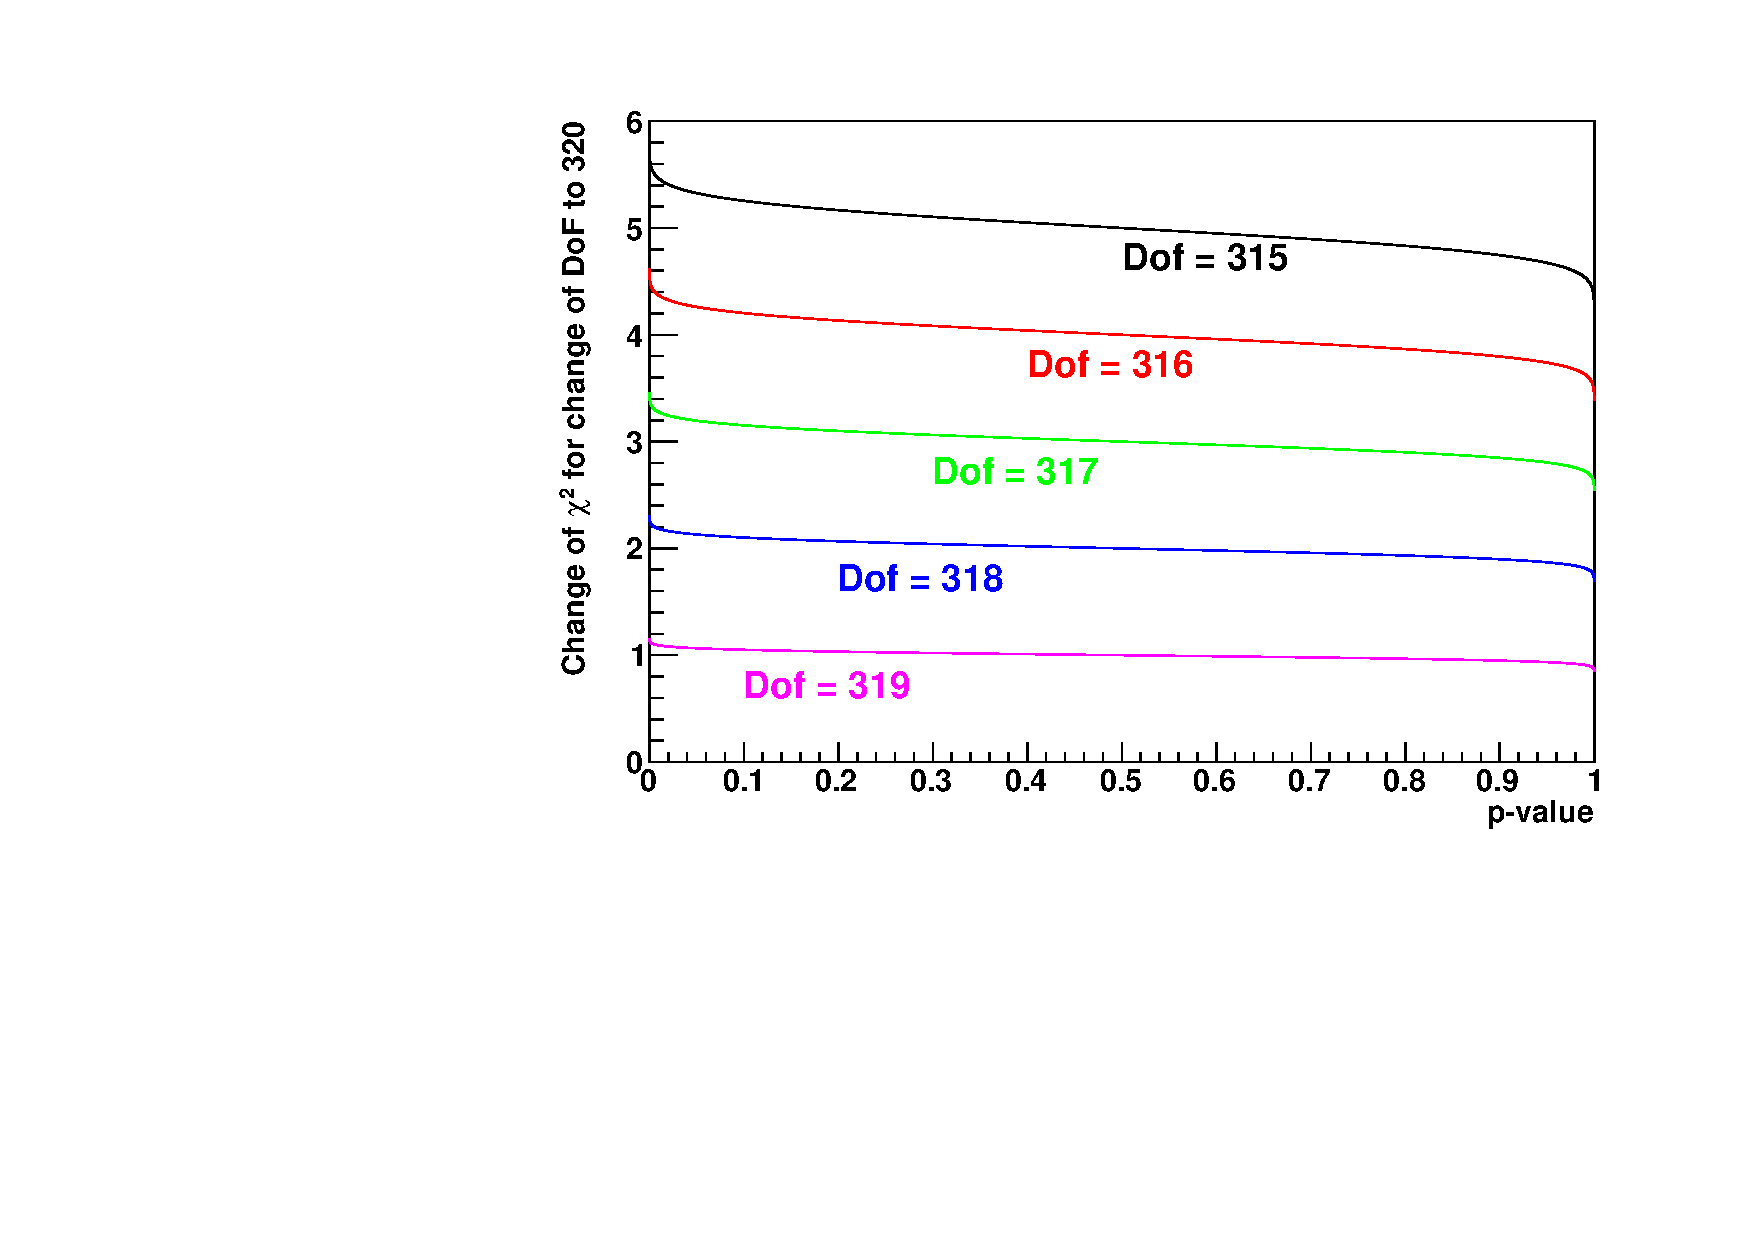
\includegraphics[width=0.45\textwidth]{correction/DeltaChiSq1.pdf}
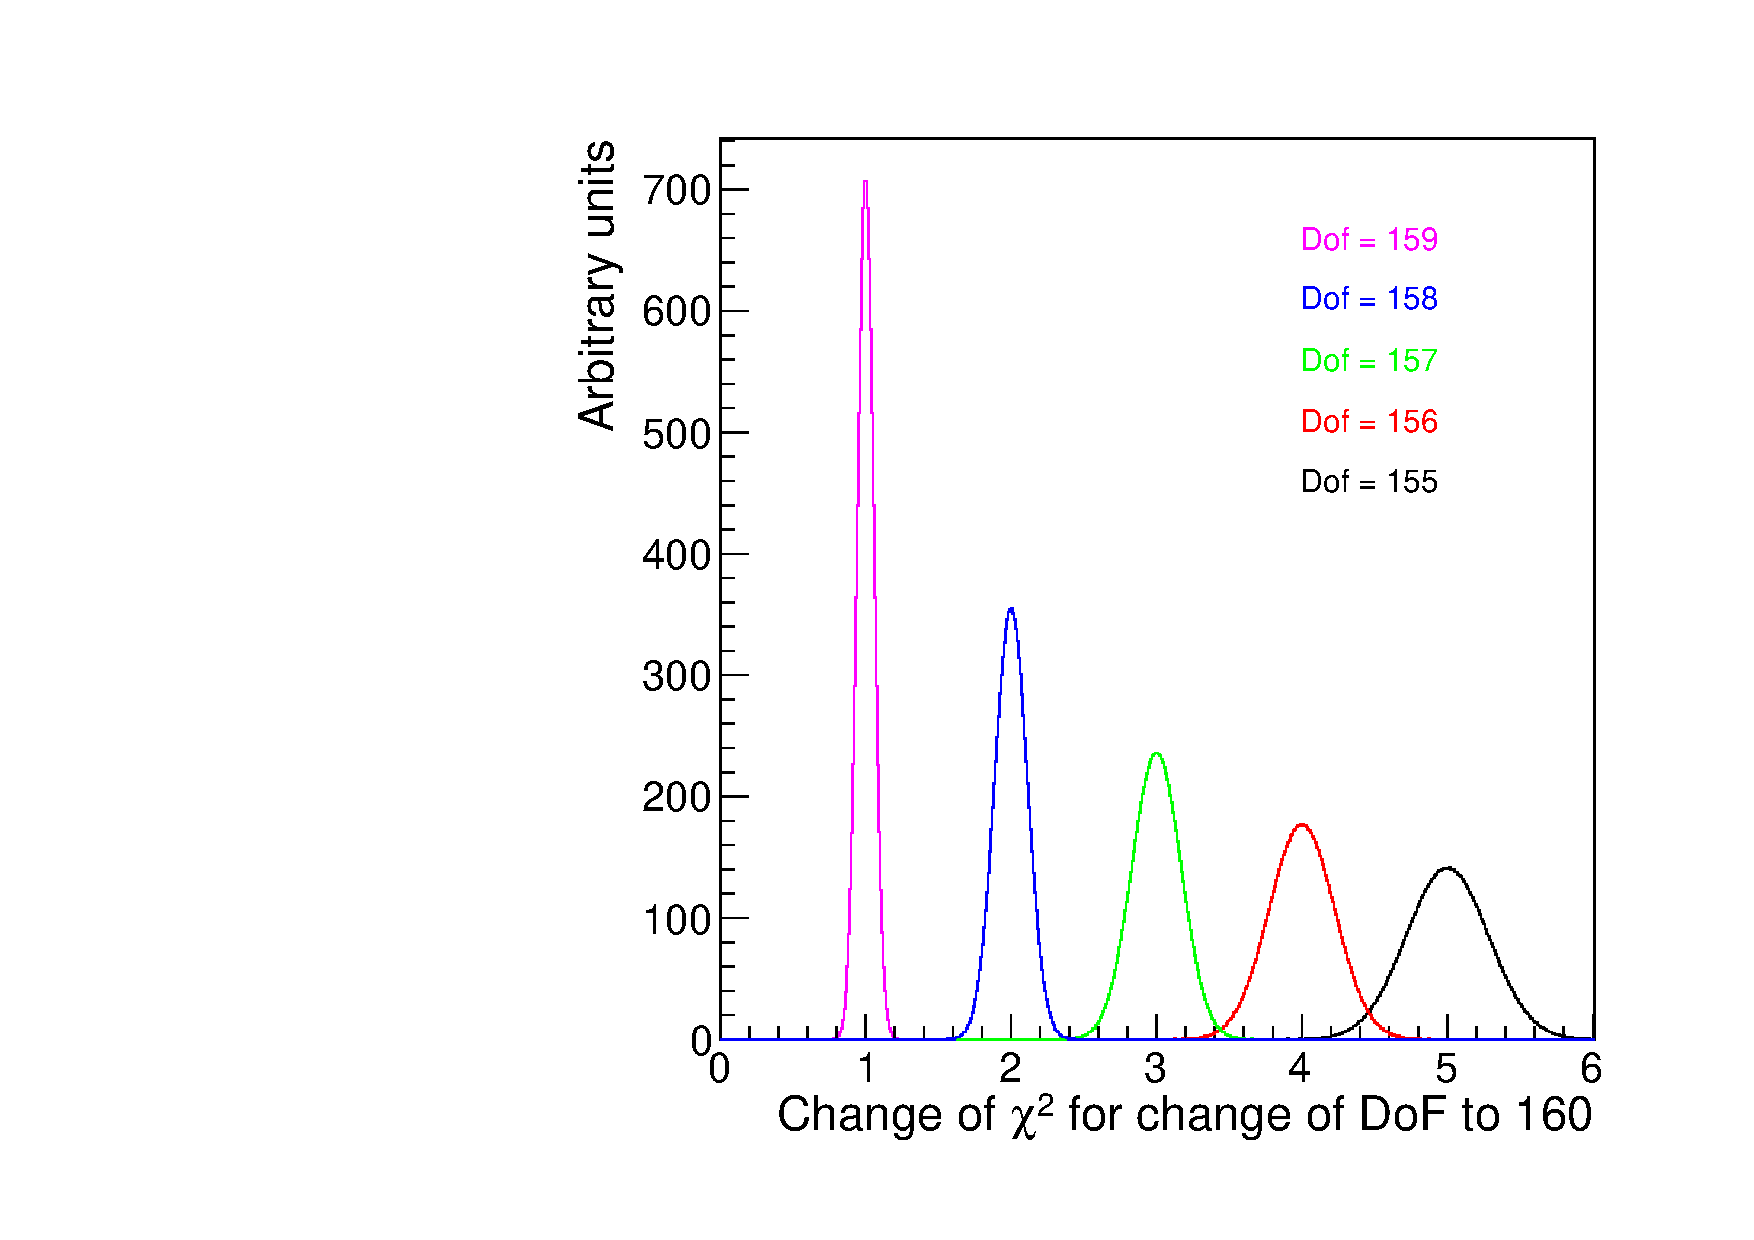
\includegraphics[width=0.45\textwidth]{correction/DeltaChiSq2.pdf}
\caption{Change of $\chi^2$ when correcting for between one and five parameters
in a fit with 160 bins. The change to the $\chi^2$ as a function of the
original p-value is shown on the left. The distribution of the change of
the $\chi^2$ assuming a flat p-value distribution is shown on the right.}
\label{fig:correction:DeltaChiSq}
\end{figure}


\item %[Akaike]
The Akaike basic formula for very large sample sizes is
\begin{displaymath}
\Lambda_{\mathrm{corr}} = \textrm{\nll} + 2N_{\rm par}
\end{displaymath}
%The resulting value of $A$ is considered here as the corrected \nll,
so the correction is simply $ 2N_{\rm par}$ and
hence is twice as big as the approximate p-value correction.
For finite samples, then it is modified to
\begin{displaymath}
\Lambda_{\mathrm{corr}}
= \textrm{\nll} + 2N_{\rm par}  + \frac{2N_{\rm par}(N_{\rm par}+1)}{n-(N_{\rm par}+1)}
= \textrm{\nll} + \frac{2N_{\rm par}}{1-(N_{\rm par}+1)/n}
\end{displaymath}
where $n$ is the sample size, i.e. the number of bins (for a binned likelihood
fit) or events (for an unbinned likelihood fit). For large $n$, the original
formula is clearly regained. This can be used for binned or unbinned fits.
Also the correction does not depend on the \nll value and
so is a simple shift of
the whole profile curve, without changing its shape.
Hence, it also has no effect on coverage.
\end{enumerate}

\subsection{Function definitions}
\label{sec:correction:functions}
The fit functions which were used are the two-parameter functions listed in
Section~\ref{sec:functions:function} and higher order generalisations of
these. Specifically, these are
\begin{enumerate}
\item
``Power law''; $f(x) = \sum_{i=0}^N p^{a}_{i} x^{p^{b}_{i+1}}$.
\item
``Exponential''; $f(x) = \sum_{i=0}^N p^{a}_{i} e^{p^{b}_{i+1}x}$.
\item
``Laurent''; $f(x) = \sum_{i=0}^N p_i/x^n$.
\item
``Polynomial''; $f(x) = \sum_{i=0}^N p_i x^i$.
\end{enumerate}
The Laurent function values of $n$ used for $i=0,1,2,3,4,5\dots$ are
$n=4,5,3,6,2,7\dots$, meaning they are grouped around the original
two $n$ values of 4 and 5 as used throughout Section~\ref{sec:functions}.
Note the power law and exponential functions can only have even numbers of
parameters, i.e. $N_{\rm par}=2N$, while the Laurent and polynomial functions
can have both even and odd numbers, i.e. $N_{\rm par}=N$.


\subsection{Example case}
\label{sec:correction:example}

The functions listed above were fit to the original dataset for values of
$2 \le N_{\rm par} \le 6$; this resulted in three fits for the power law and
exponential functions, and five fits for the Laurent and polynomial functions.
The profiles for each of these function fits are shown in
figure~\ref{fig:correction:profiles}, for the example case of
applying the approximate p-value correction to the \nll of one unit per
background function parameter.

For this case, the lowest corrected \nll value is still given by the
two-parameter power law function and so gives an identical central value
to that described in Section~\ref{sec:functions:example}. The lowest corrected
\nll value for $\mu < 0.55$ is also again given by the two-parameter exponential
function, also as for the previous case.
Indeed, comparison to figure~\ref{fig:functions:profiles} shows that the
minimum values of the corrected \nll for low $\mu$
are simply two units larger here than in that figure.
However, for $1.48 < \mu < 1.68$
the $N_{\rm par}=5$ polynomial is the lowest function in the profile,
while for $\mu > 1.68$,
the $N_{\rm par}=6$ polynomial is lowest.
Hence, the envelope is formed from four different functions in this
case. Figure~\ref{fig:correction:profiles} also shows the 68.3\% and
95.4\% confidence intervals which would be determined from the
profile envelope. The 68.3\% region is identical to that found using
just the two-parameter functions (see Section~\ref{sec:functions:example}), but
when including higher order functions, the 95.4\% confidence interval
on $\mu$ is $-0.18 < \mu < 2.11$,
i.e. it is extended to higher $\mu$
due to the influence of the higher order polynomial functions providing a
reasonable description of the data.
%The central value is unchanged since the lowest order power law
%best desribes the data when including a penalty for using additional parameters in the fit.

\begin{figure}[tbp]
\centering
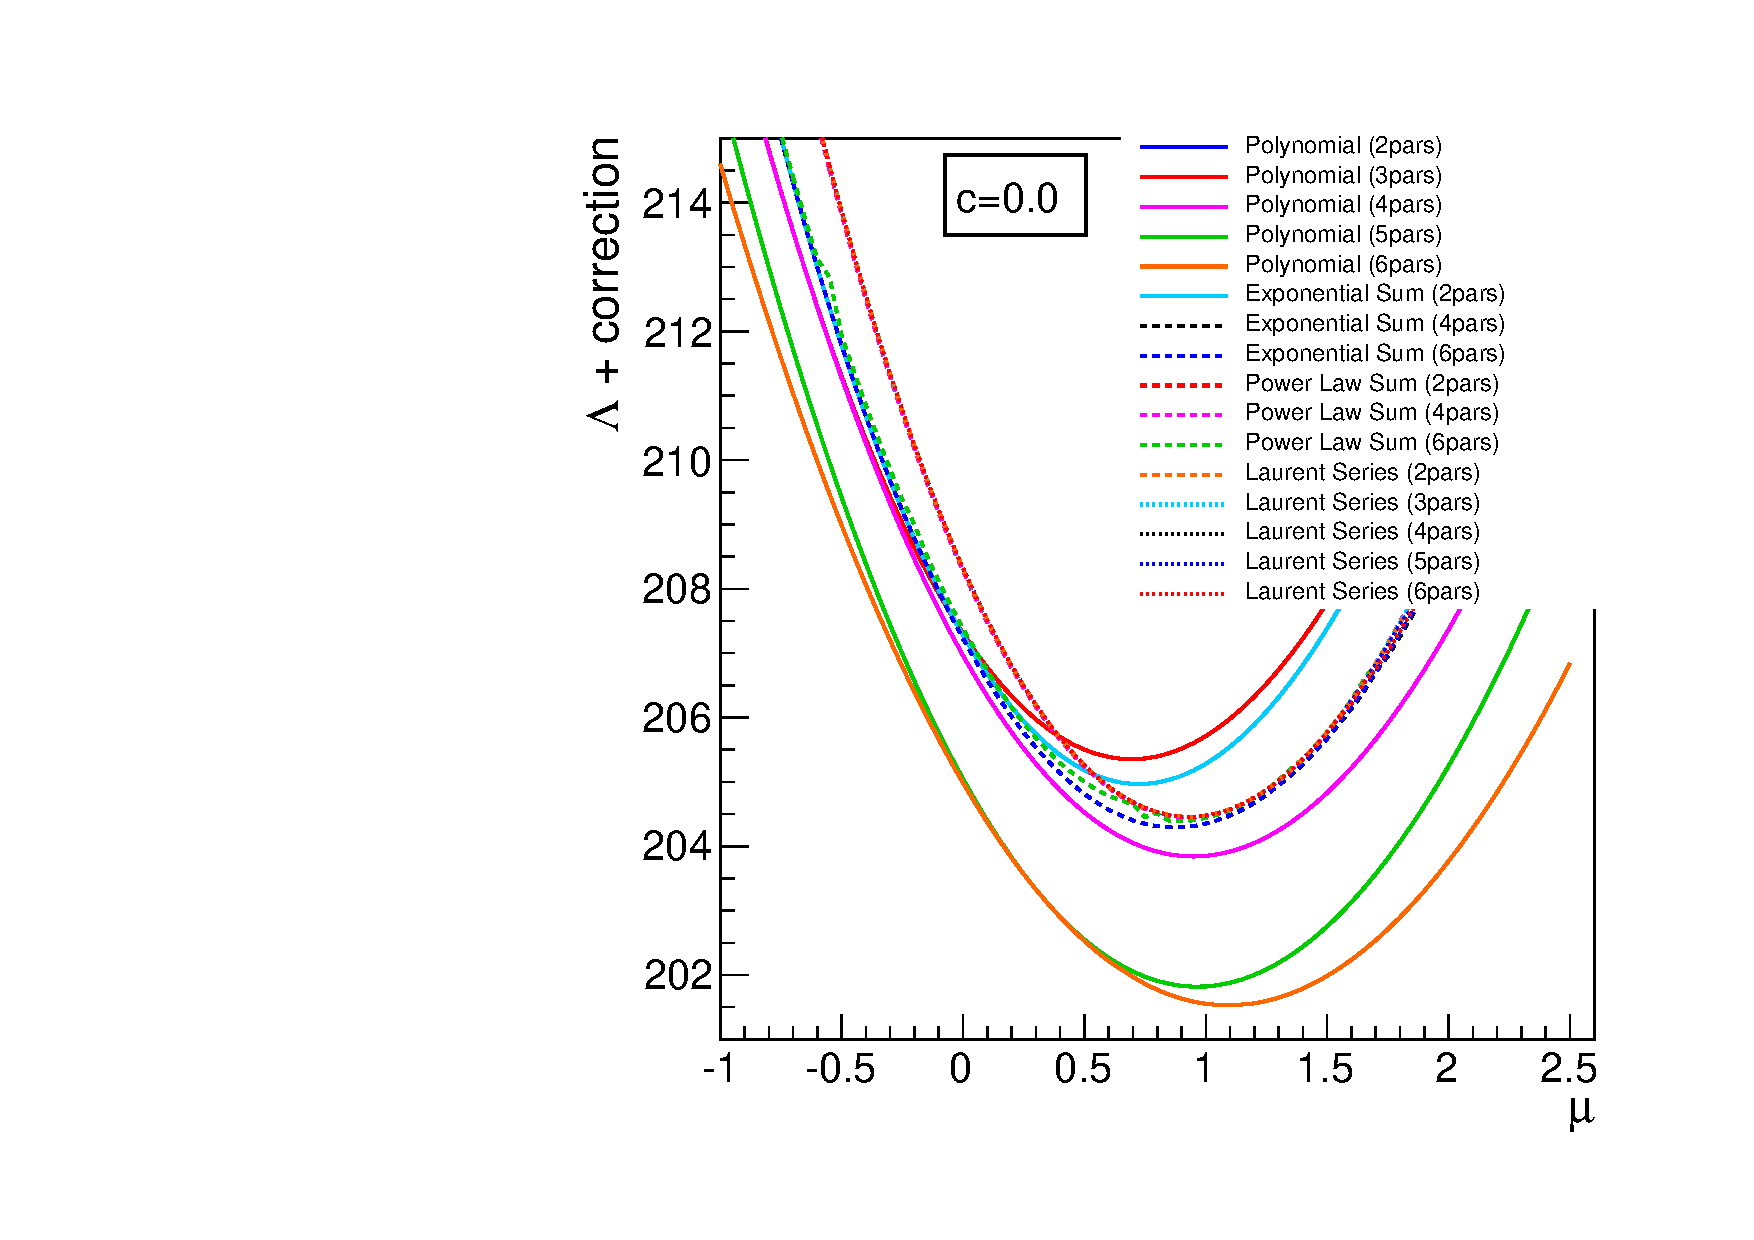
\includegraphics[width=0.45\textwidth]{{correction/ProfilesAllOrders0.0}.pdf}
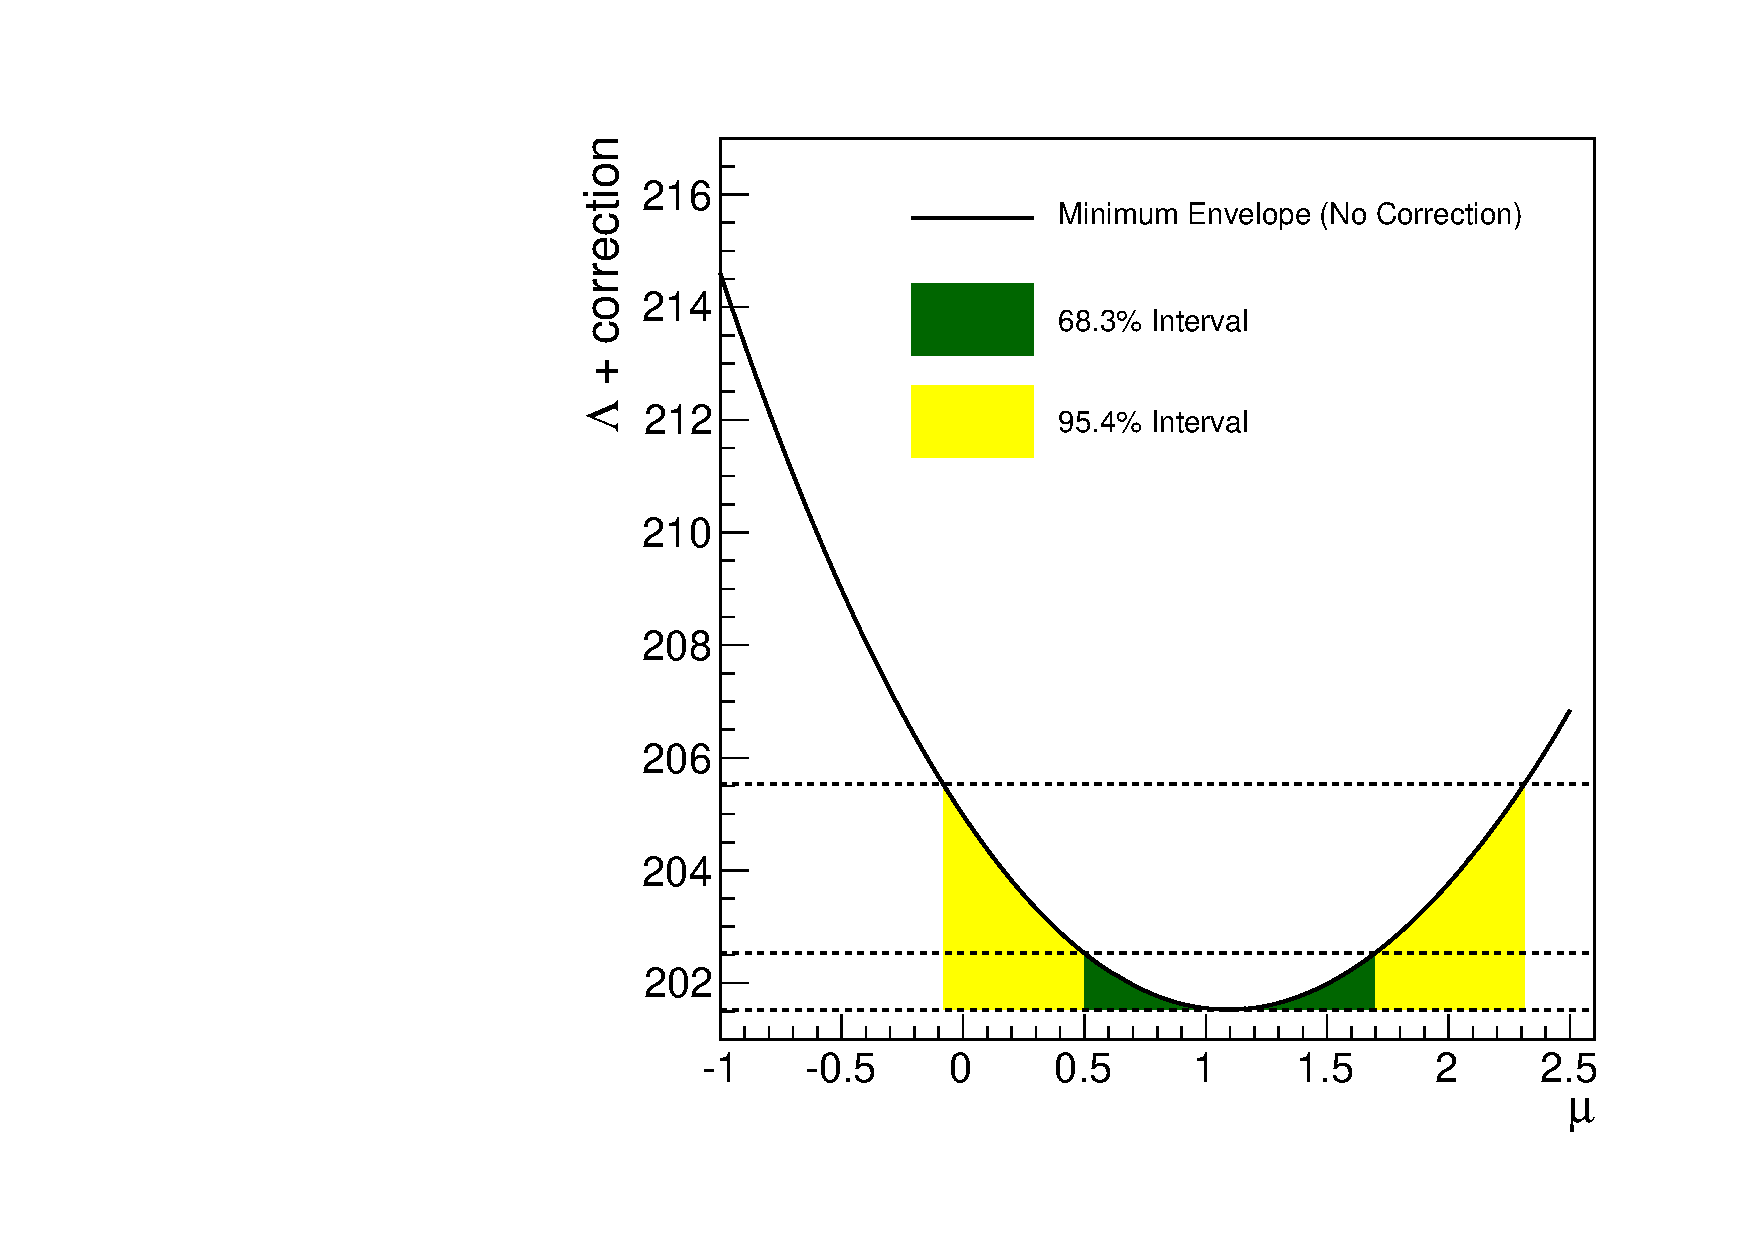
\includegraphics[width=0.45\textwidth]{{correction/EnvelopeAllOrders0.0}.pdf} \\
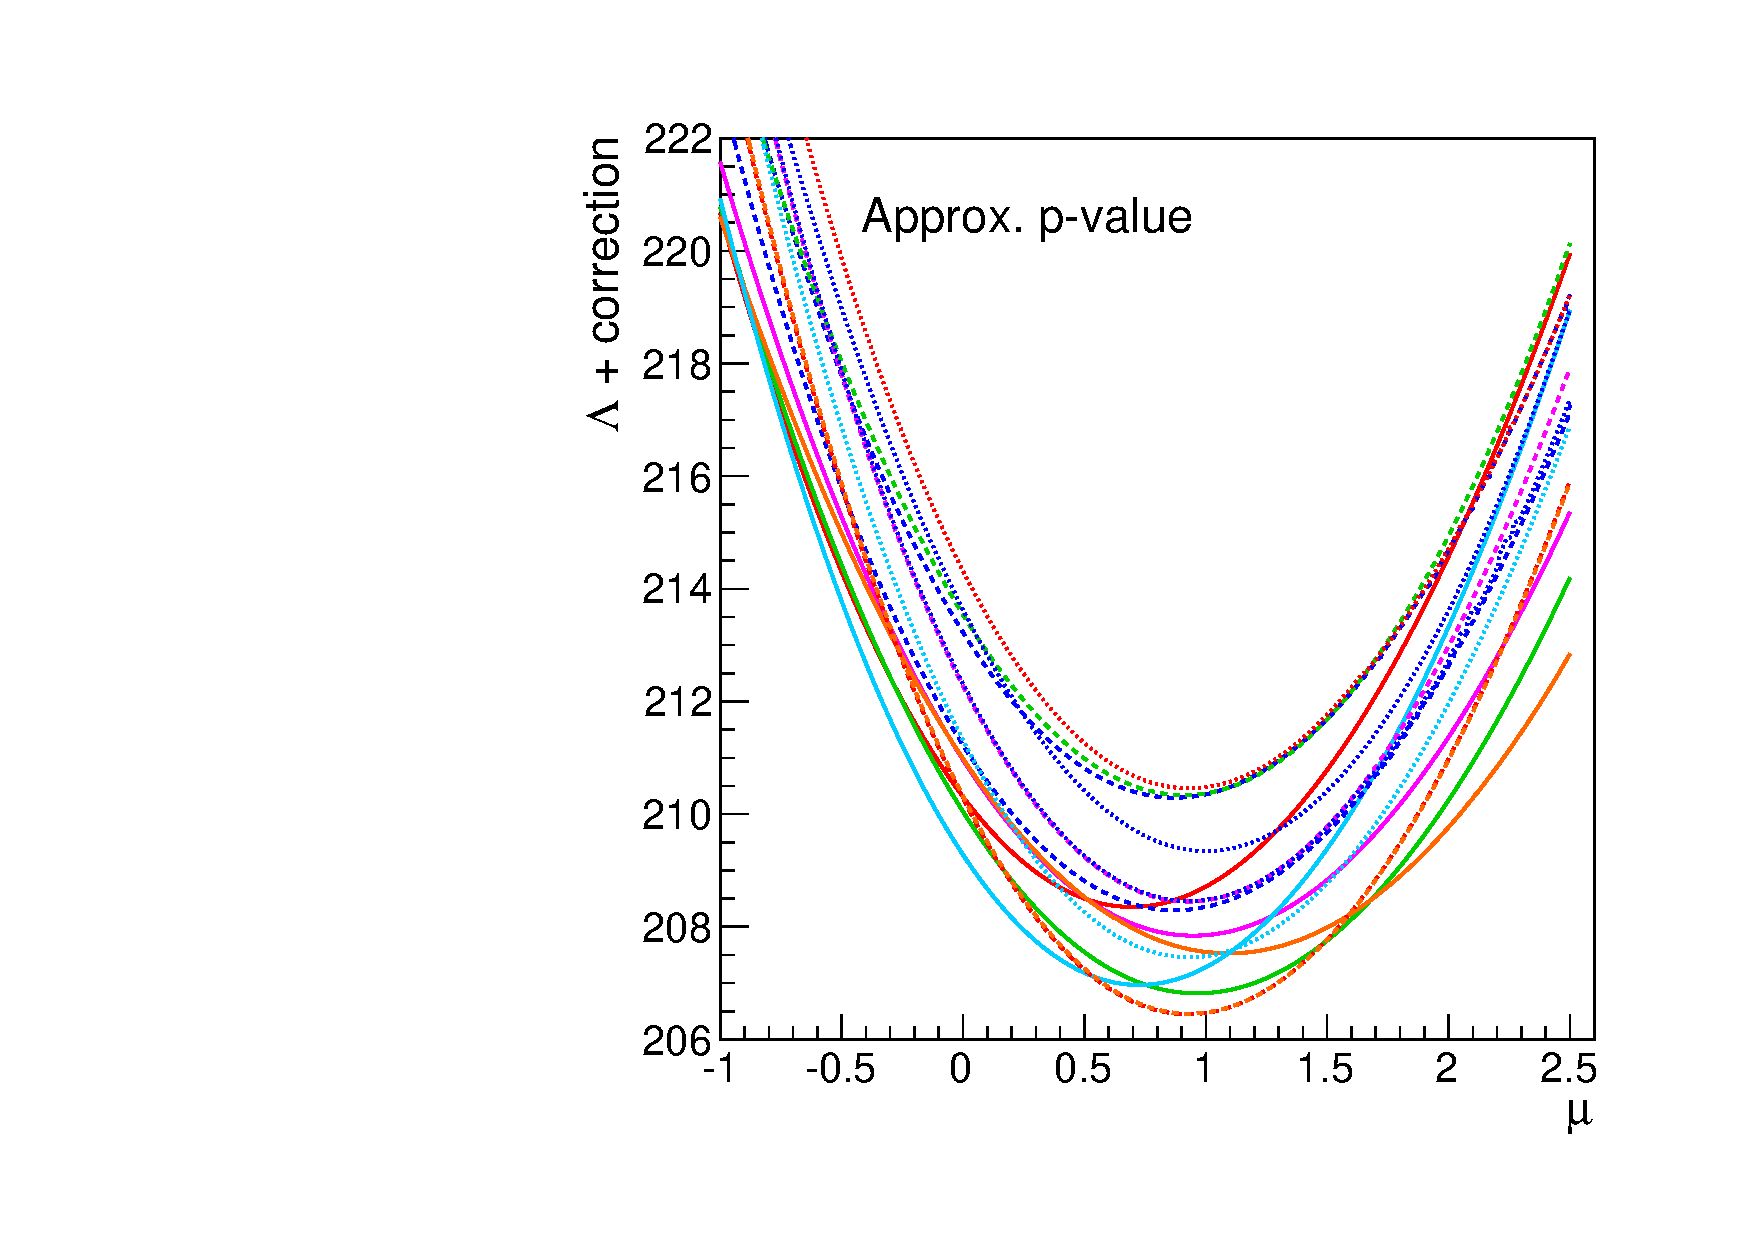
\includegraphics[width=0.45\textwidth]{{correction/ProfilesAllOrders1.0}.pdf}
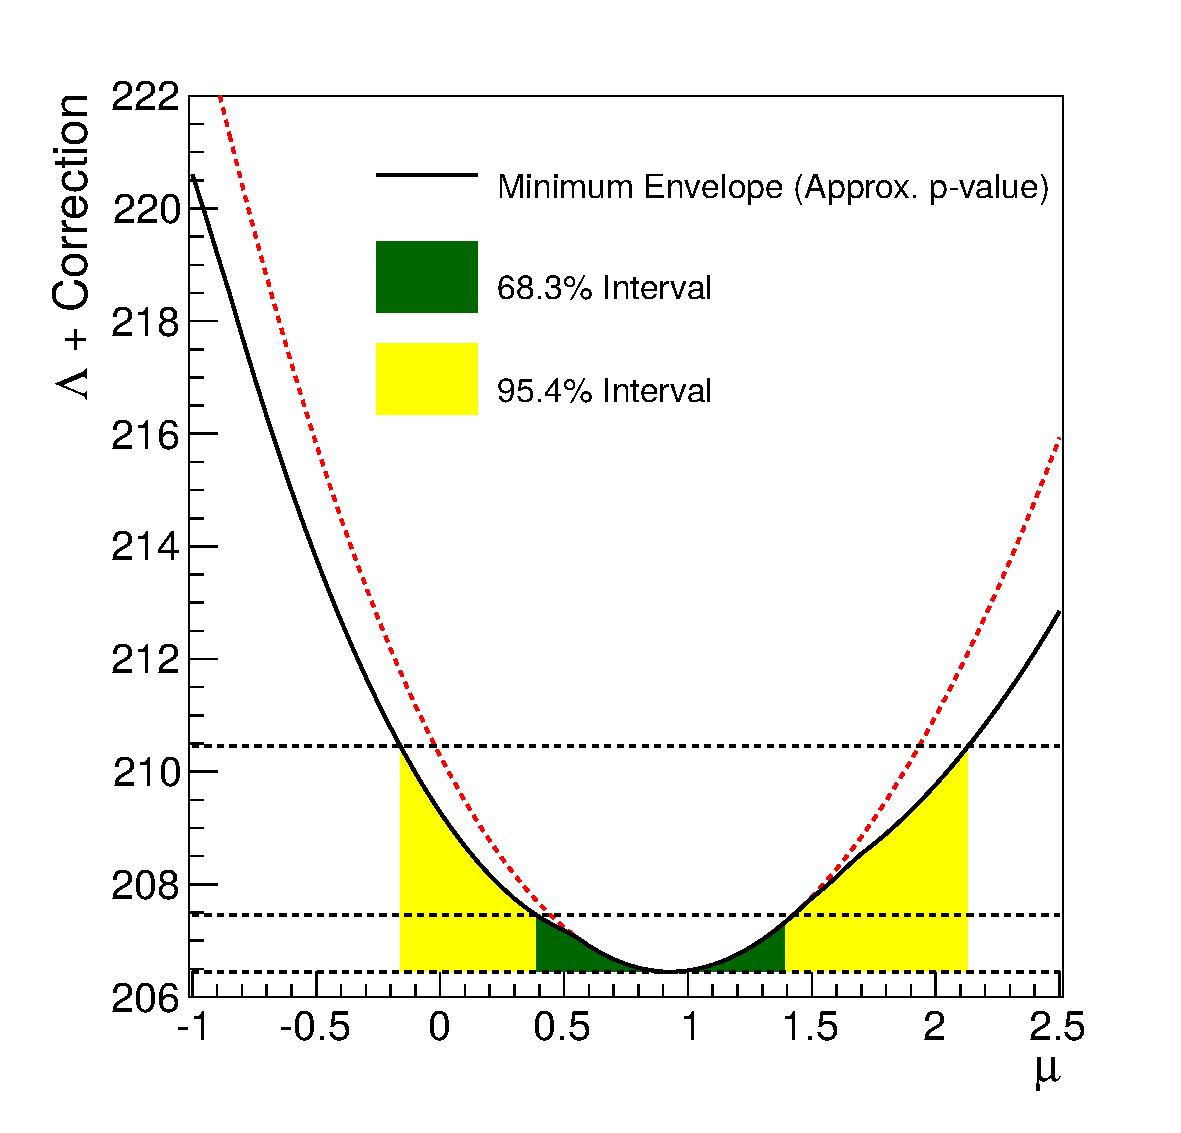
\includegraphics[width=0.45\textwidth]{{correction/EnvelopeAllOrders1.0}.pdf} \\
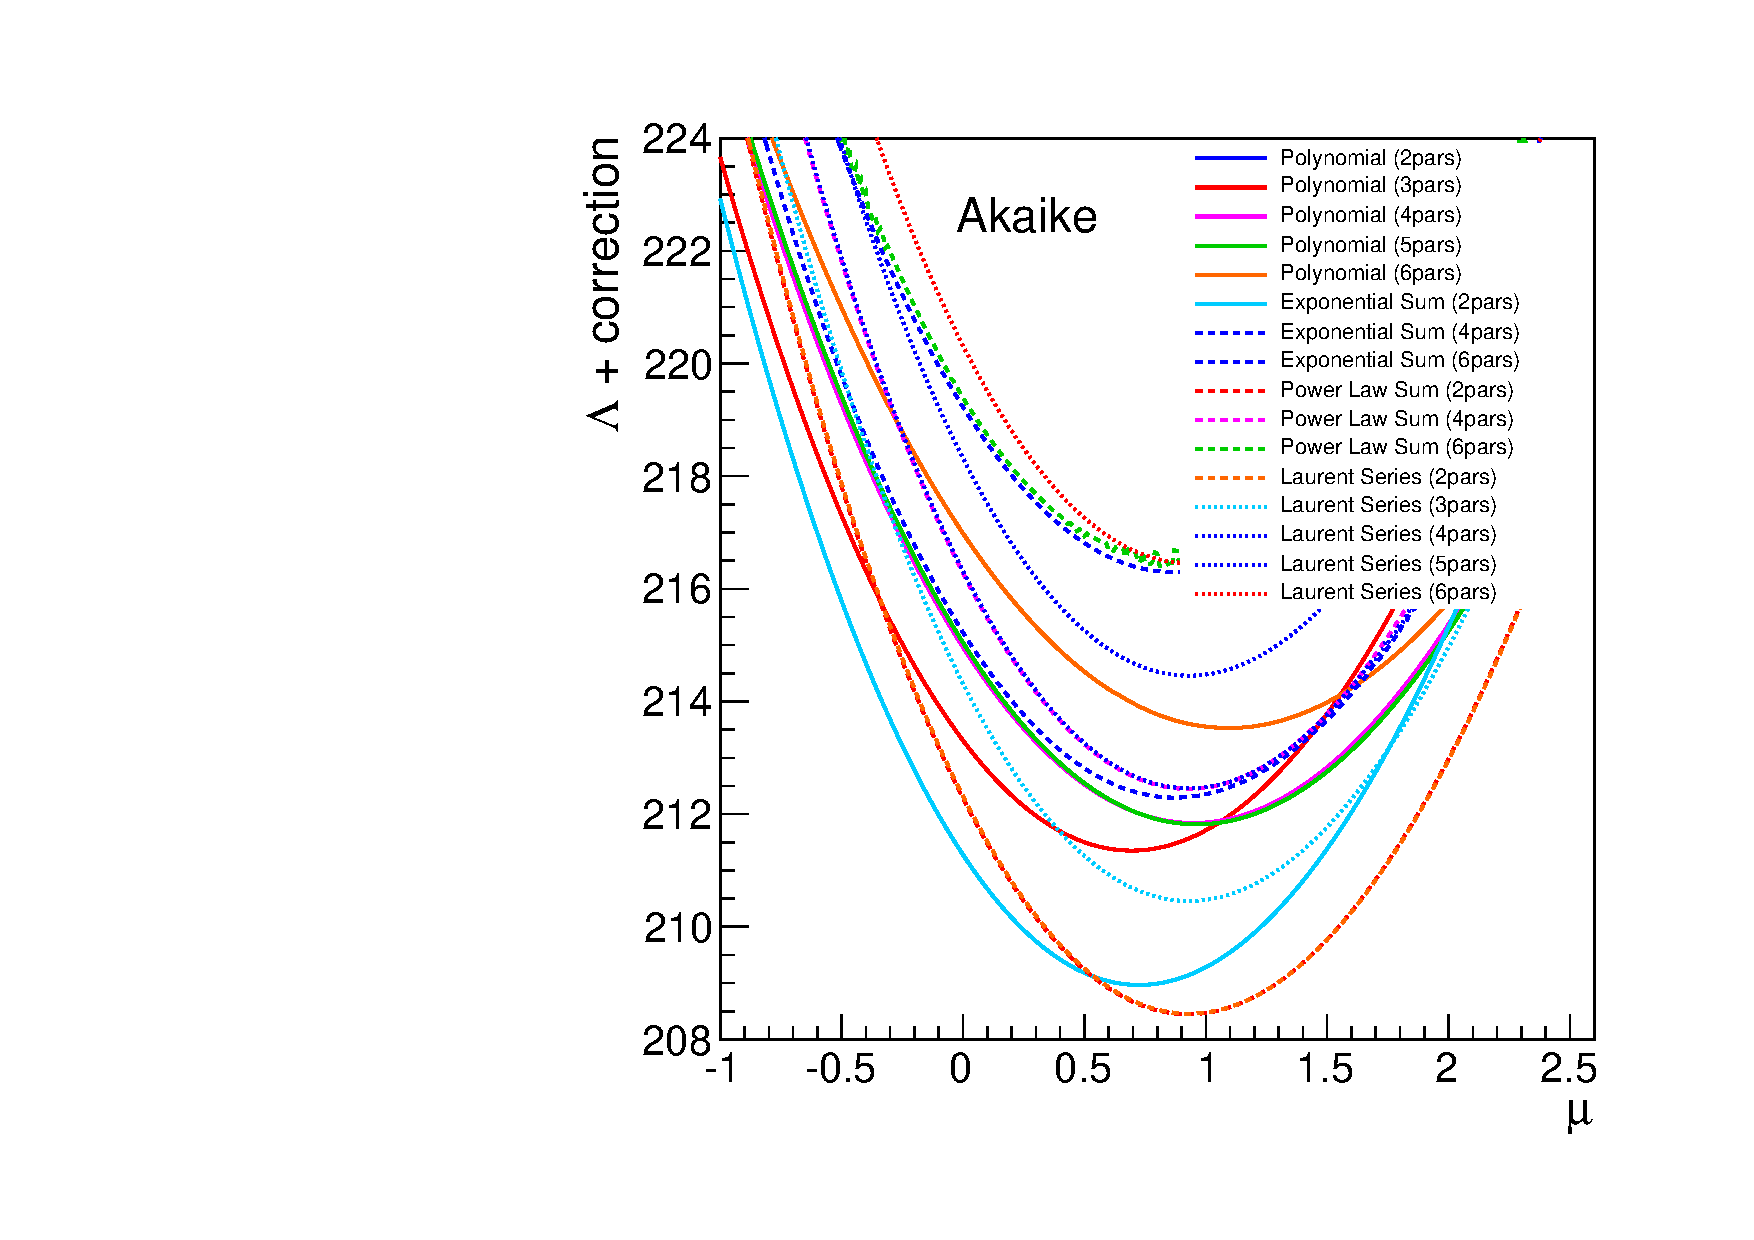
\includegraphics[width=0.45\textwidth]{{correction/ProfilesAllOrders2.0}.pdf}
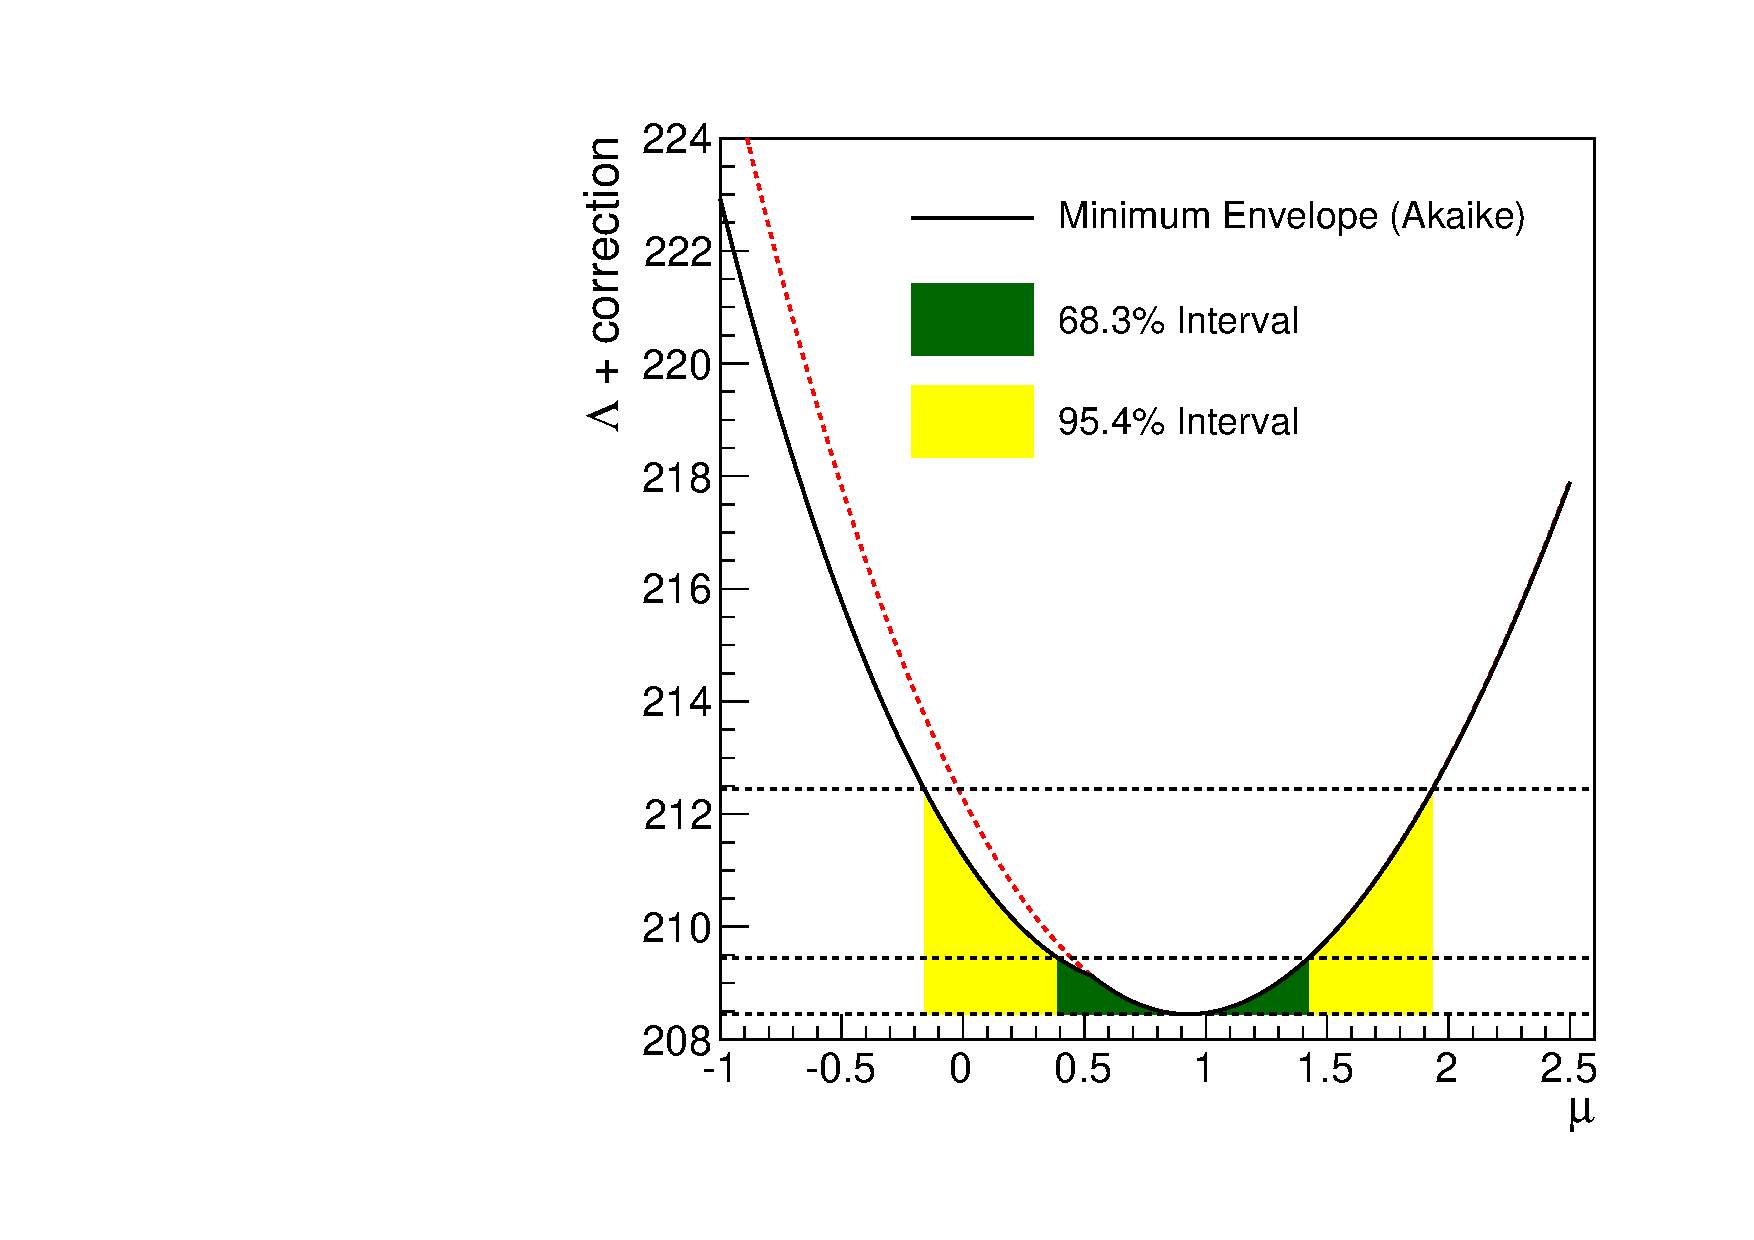
\includegraphics[width=0.45\textwidth]{{correction/EnvelopeAllOrders2.0}.pdf}
\caption{Left: Profile \nll scans for all of the functions considered. The \nll values for each profile have been corrected by no units (top), one unit per background function parameter (middle) and two units per background function parameter (bottom). The labels indicate the function and the value of $N_{\rm par}$. Right: Minimum envelope of the functions considered accounting for the correction of either 0, 1 or 2 per background parameter. The \nll scan when only considering the best fit function is shown in red.}
\label{fig:correction:profiles}
\end{figure}

\begin{figure}[htp]
\centering
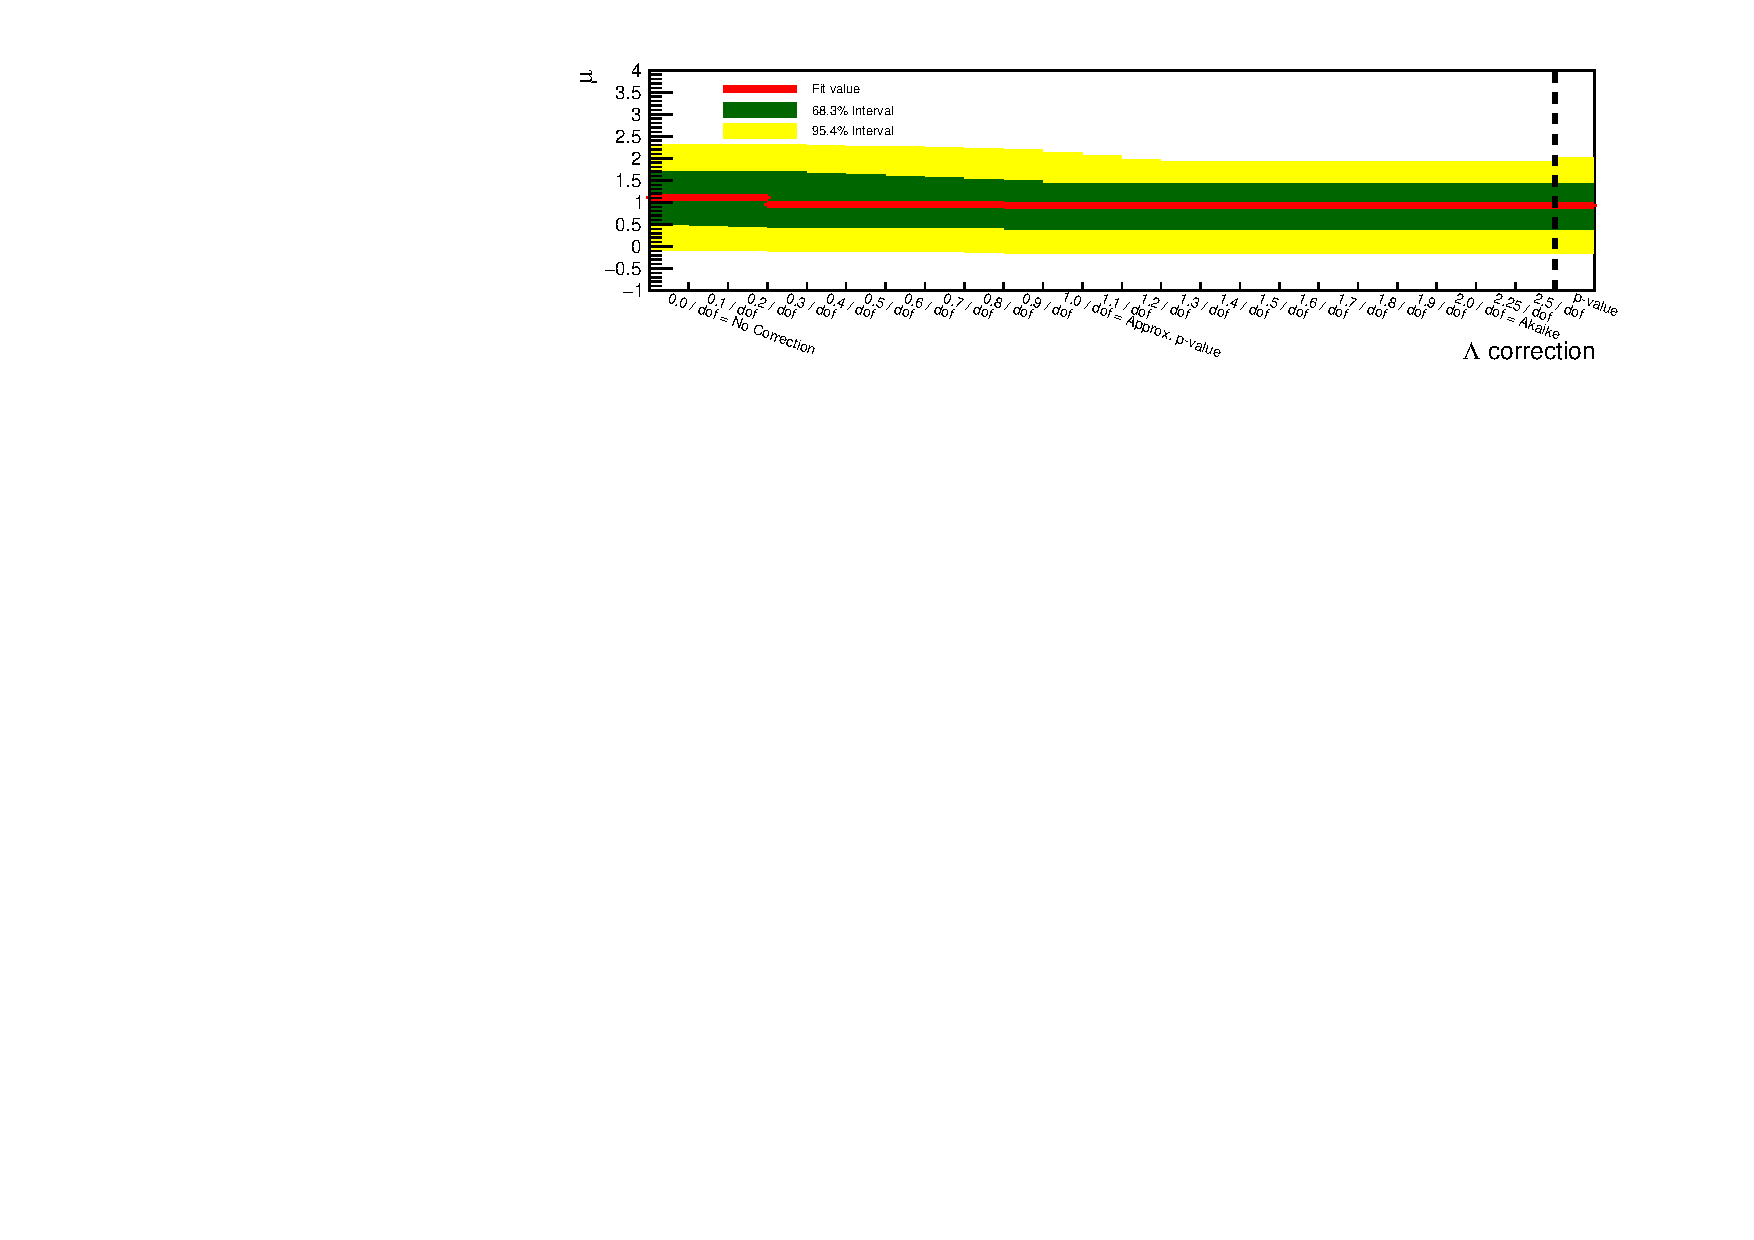
\includegraphics[width=0.65\textwidth]{correction/correction.pdf}
\caption{The best fit value of the signal strength, $\mu$, and its uncertainty when fitted to the dataset as a function of the correction apllied per background parameter.}
\label{fig:correction:correction}
\end{figure}


%RELATION TO BIAS WHEN USING FUNCTION A TO FIT FUNCTION B? ASIMOV?

%\subsection{Toy generation}
%\label{sec:correction:toys}

%EXTRA COMPLICATION WITH BAYESIAN AND FREQUENTIST MIXTURES OF NORMALISATION

\subsection{Bias and coverage dependence on correction}
\label{sec:correction:bias}

In a similar way to Section~\ref{sec:functions:coverage}, toy datasets
were generated using various individual functions and also the best fit
functions for each $\mu$ value. The individual functions chosen were those
which gave the lowest corrected \nll values in
figure~\ref{fig:correction:profiles}.
Figure~\ref{fig:correction:allorderbias} shows the average pull vs $\mu$
for each generating function choice, with the envelope based on the
three correction methods considered, i.e.~exact p-value, approximate p-value
and Akaike. It is seen that the exact and approximate p-value corrections give
effectively identical results. It is also found that the bias for some
generating functions can get up to a significant fraction of the error, but
that the p-value corrections always give less bias than the Akaike correction.
%
\begin{figure}[tbp]
\centering
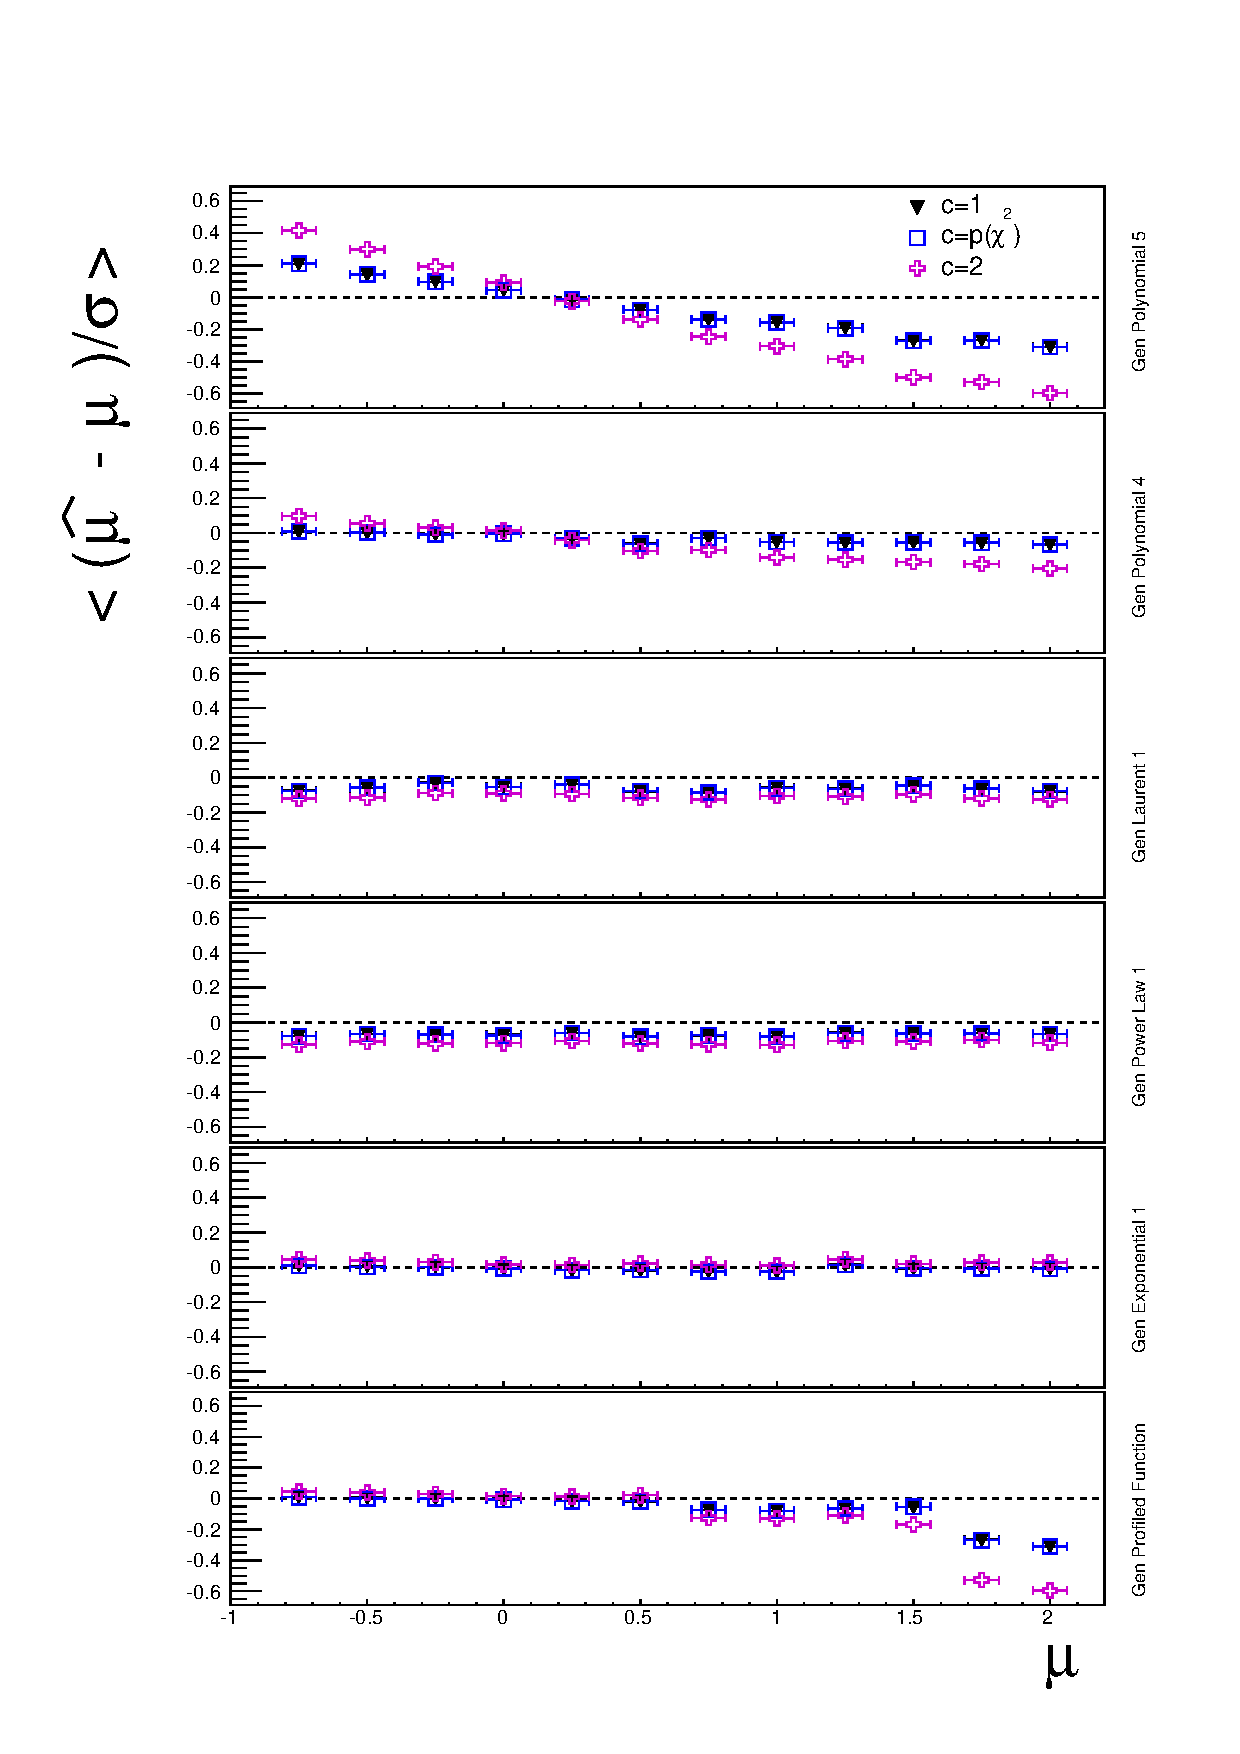
\includegraphics[width=0.48\textwidth]{correction/AllOrderFunctions_call.pdf}
\caption{Average pull when fitting using the envelope as a function of $\mu$
used to generate the signal. Each panel shows the average bias when using
a different background function for toy generation, with the functions
used being (from the top): polynomial with $N_{\rm par}=6$,
polynomial with $N_{\rm par}=5$, Laurent with $N_{\rm par}=2$,
power law with $N_{\rm par}=2$, and exponential with $N_{\rm par}=2$.
The lowest plot show the result when the best-fit function at each
value of $\mu$ is used to generate toys.
%For each plot, the results for the three correction methods are shown,
%namely the approximate p-value (``$c=1$''), exact p-value (``$c=p(\chi^2)$'')
%and Akaike (``$c=2$'').
}
\label{fig:correction:allorderbias}
\end{figure}

Similarly, figure~\ref{fig:correction:allordercoverage} shows the fraction of
times the envelope fit result was within the various \nll ranges, as used
previously in figure~\ref{fig:functions:firstordercoverage}. Again, the
coverage is reasonably good for all cases. As for the bias, the two
p-value corrections are identical and always give a better result than the
Akaike correction.
%
\begin{figure}[tbp]
\centering
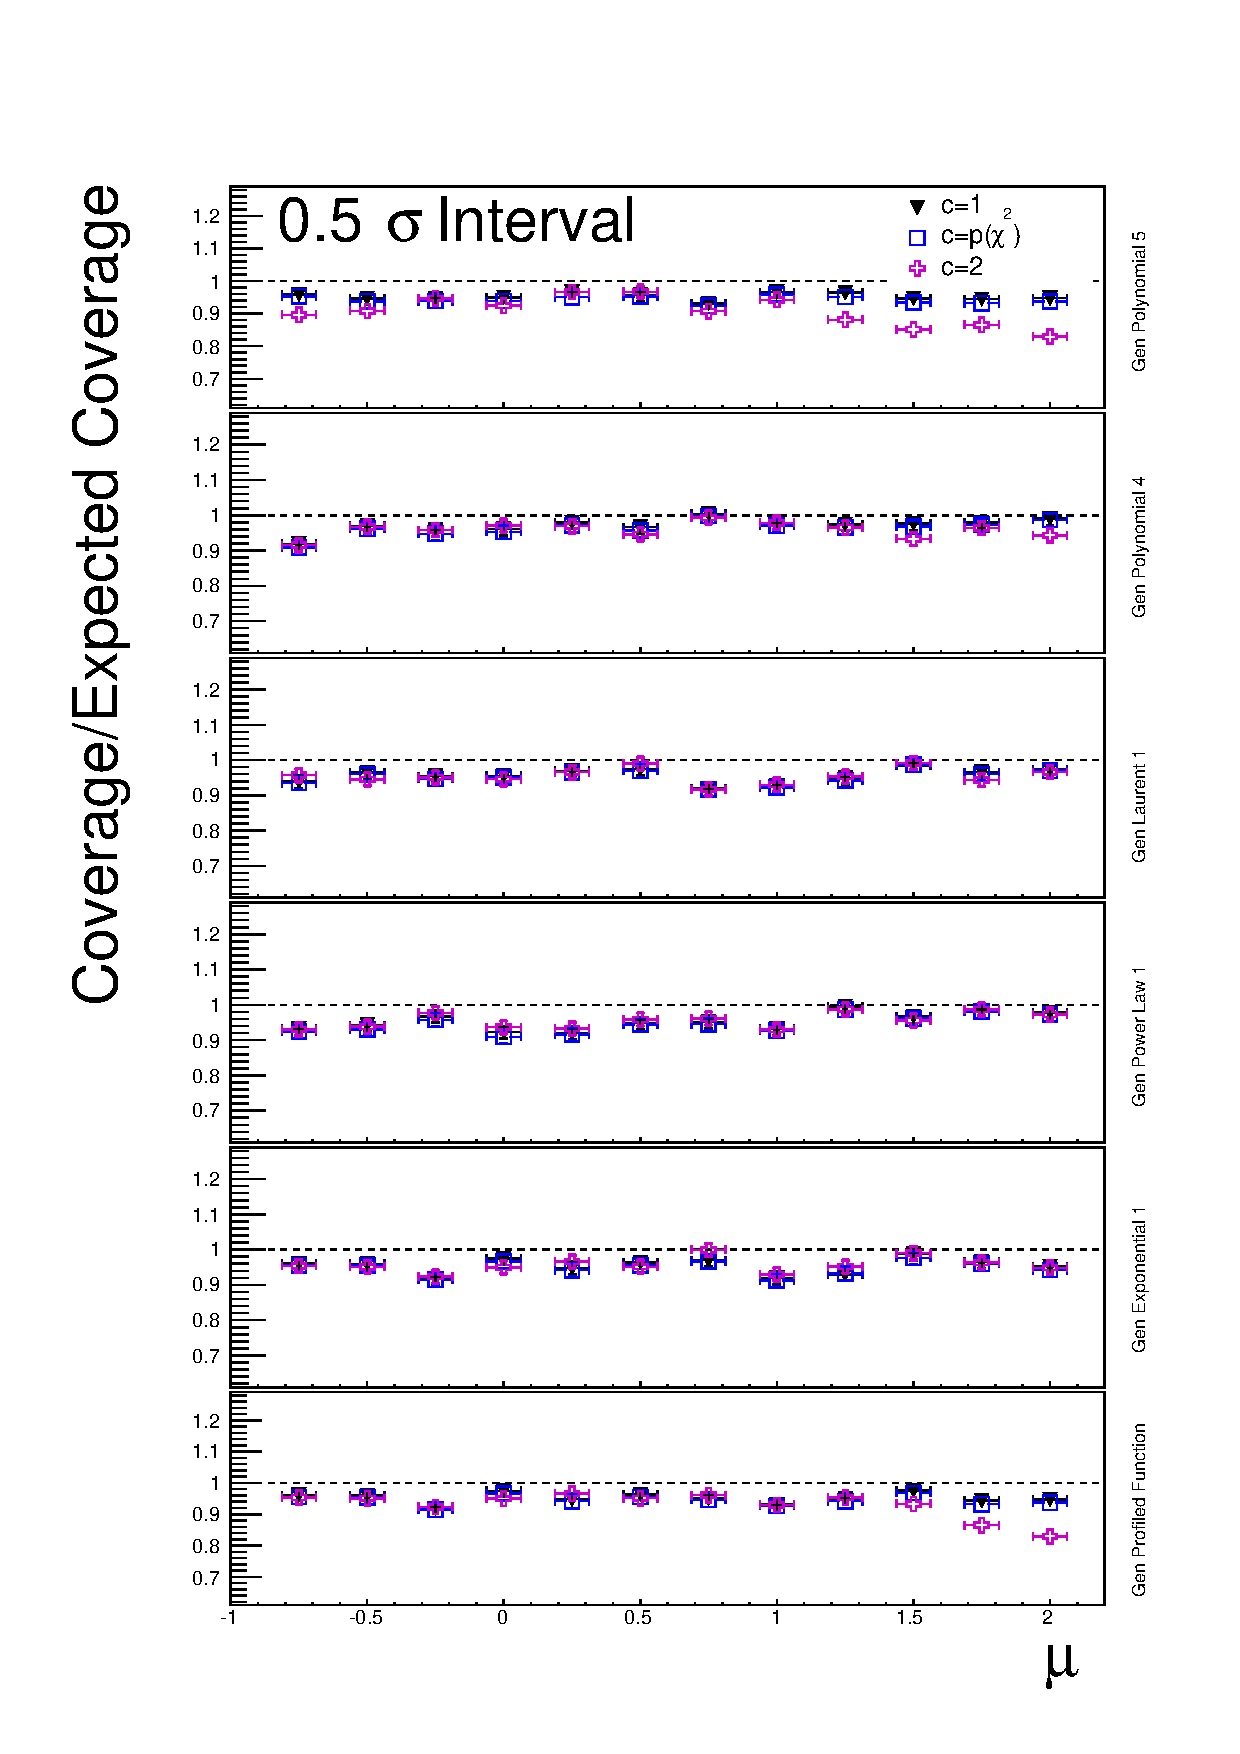
\includegraphics[width=0.45\textwidth]{{correction/AllOrderFunctions_Coverage_0.5_call}.pdf}
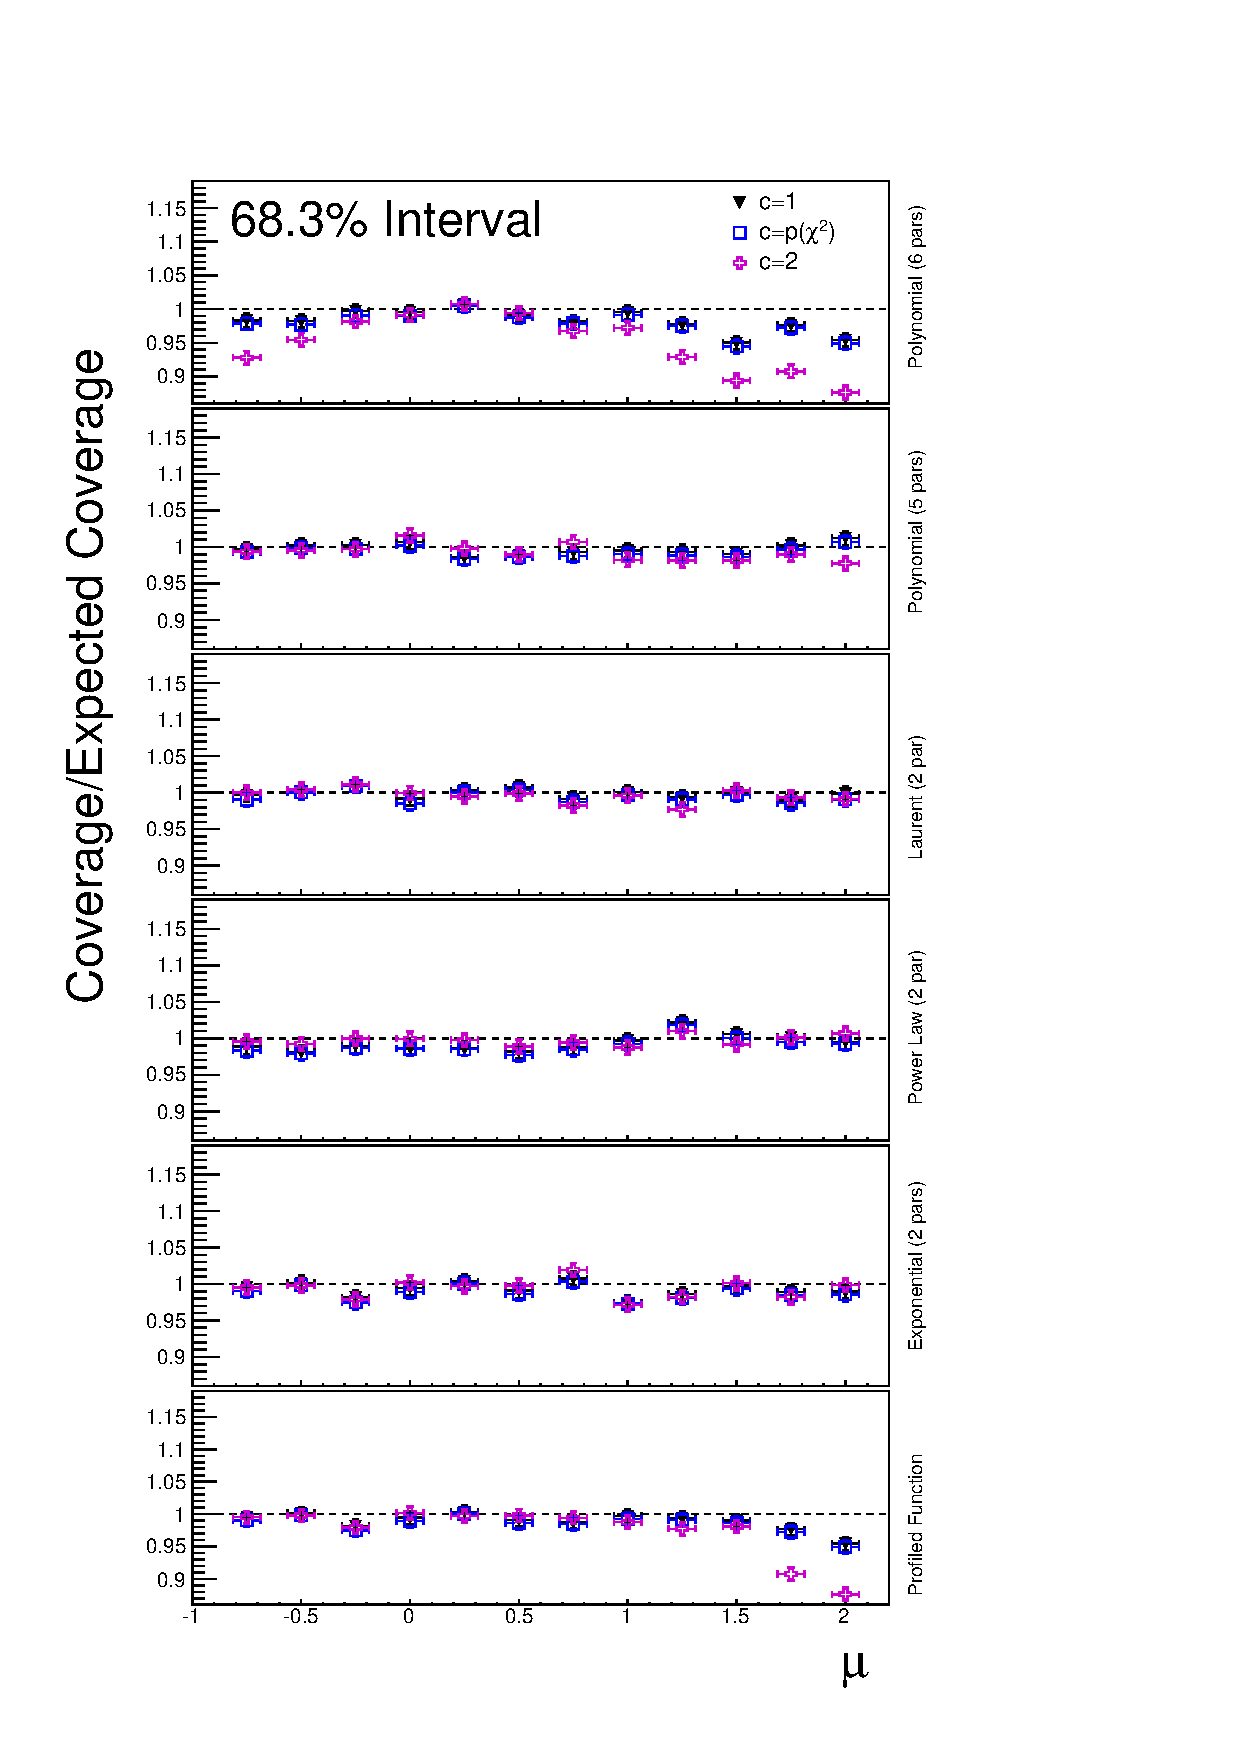
\includegraphics[width=0.45\textwidth]{{correction/AllOrderFunctions_Coverage_1._call}.pdf}\\
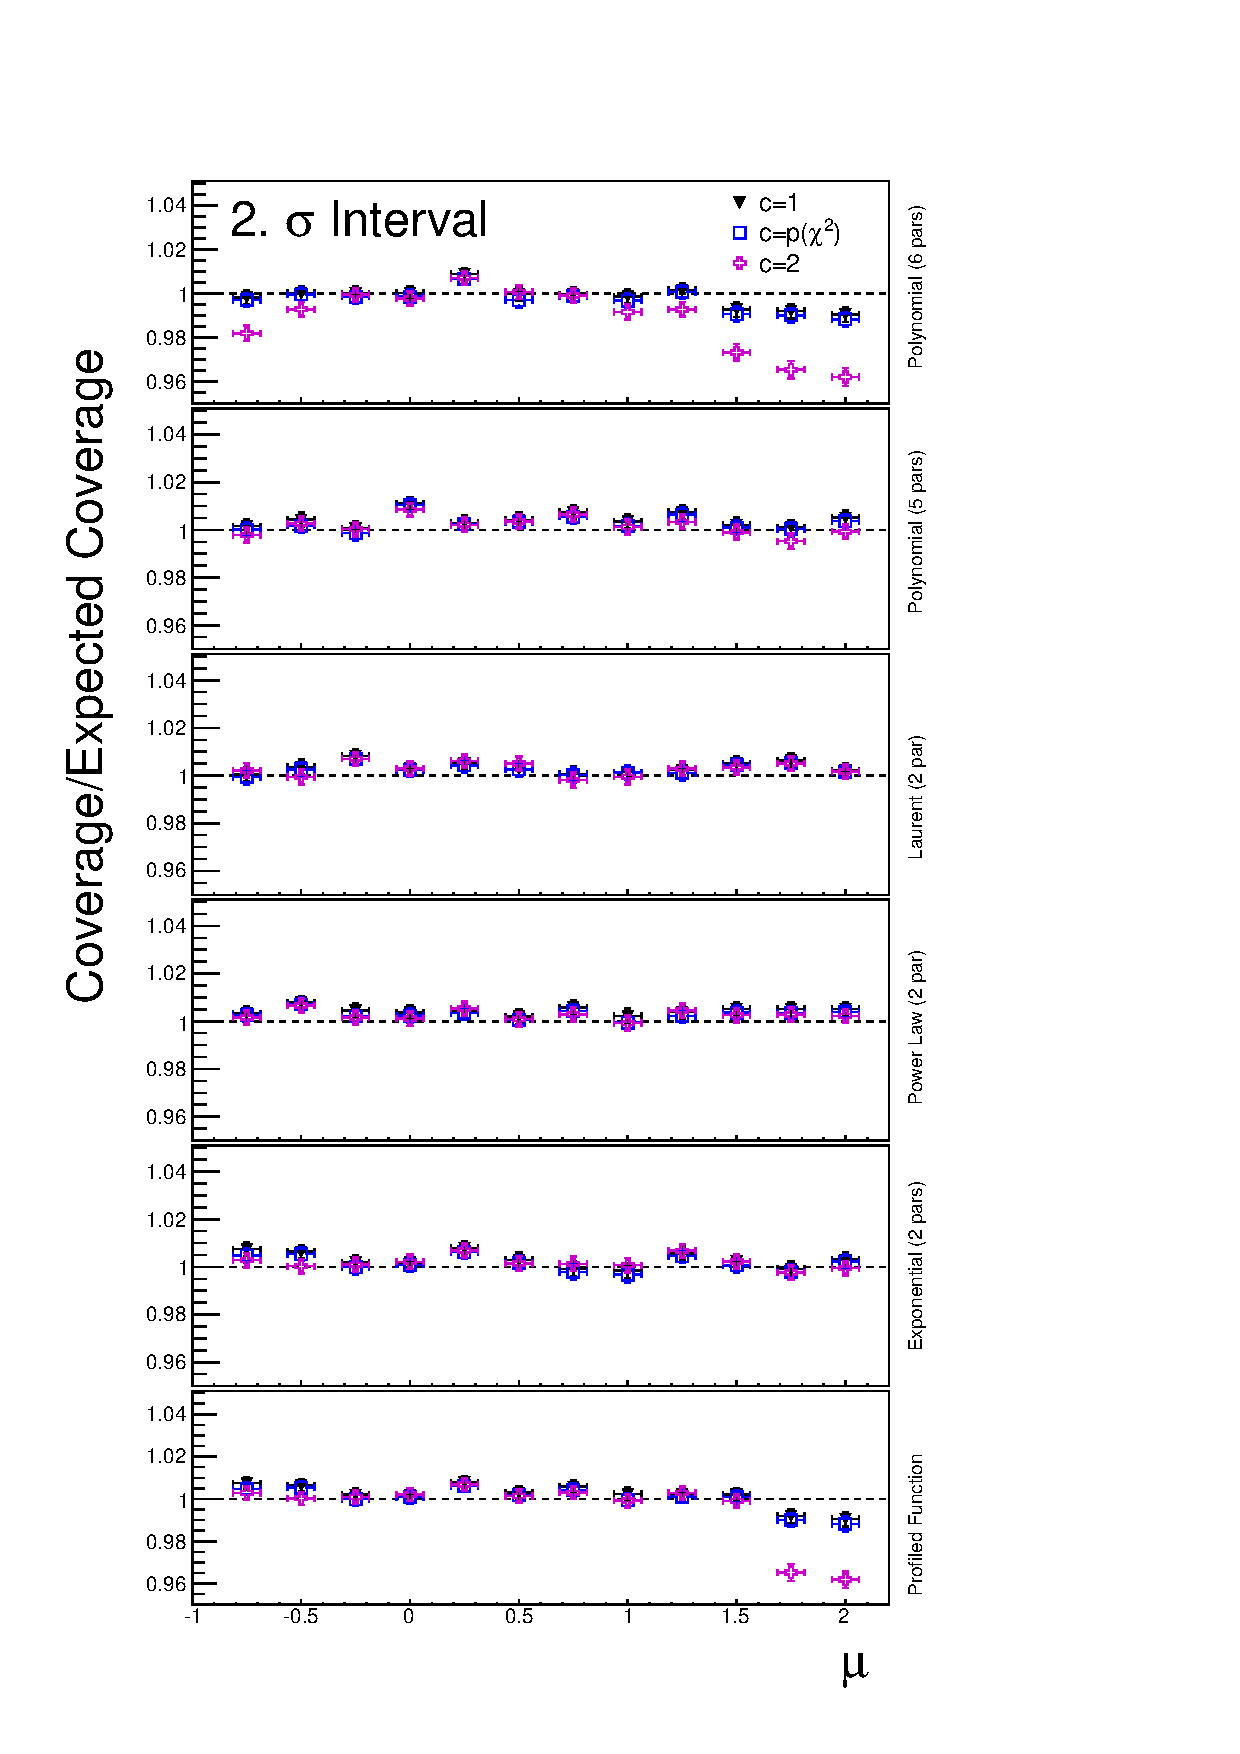
\includegraphics[width=0.45\textwidth]{{correction/AllOrderFunctions_Coverage_2._call}.pdf}
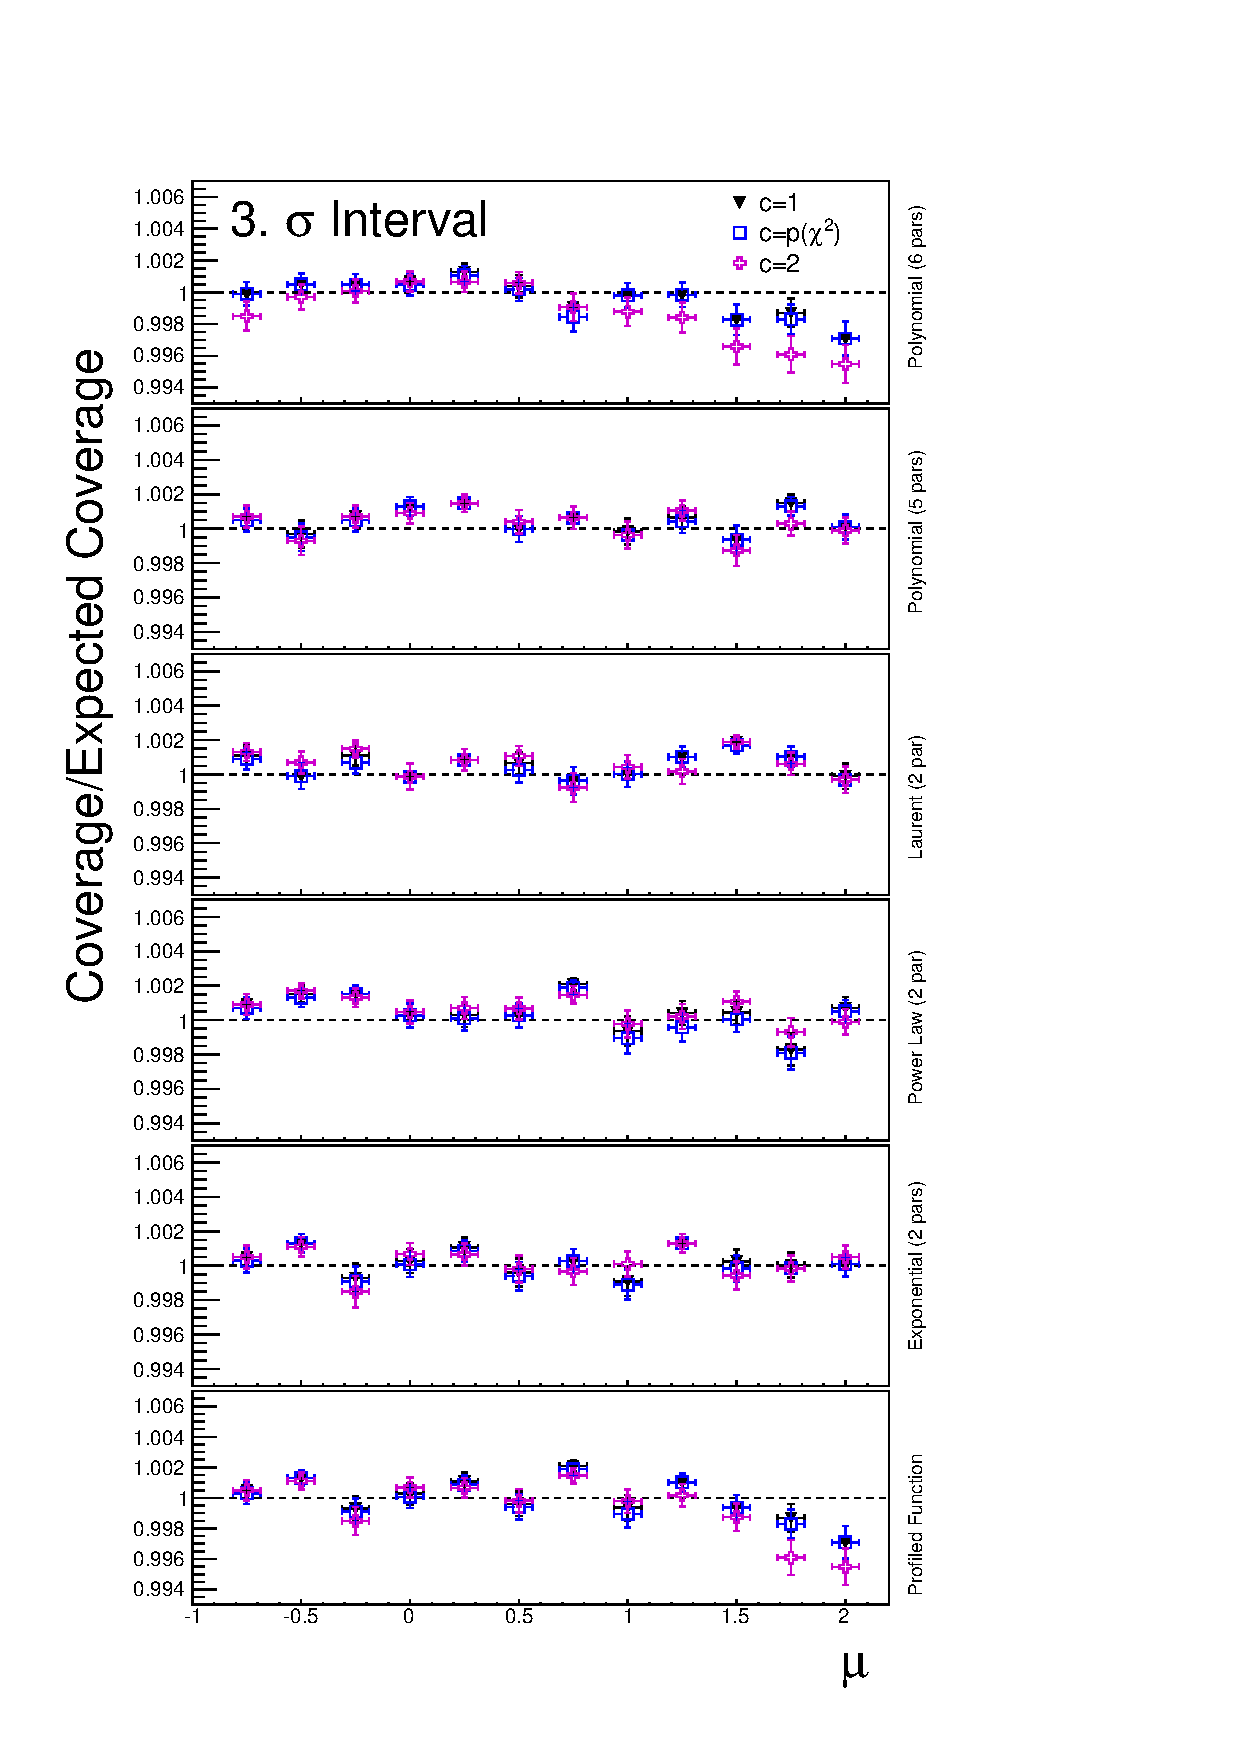
\includegraphics[width=0.45\textwidth]{{correction/AllOrderFunctions_Coverage_3._call}.pdf}
\caption{Fraction of toys in which the fitted value of $\mu$ is within the 38.3\%, 68.3\%, 95.4\% and
99.7\% intervals relative to the expected fraction for that interval
when correcting
with the different \nll correction schemes.
The results when generating with different functions and generating using the
profiled function for each value of $\mu$ are shown in the different panels.
The functions
used are (from the top): polynomial with $N_{\rm par}=6$,
polynomial with $N_{\rm par}=5$, Laurent with $N_{\rm par}=2$,
power law with $N_{\rm par}=2$, and exponential with $N_{\rm par}=2$.
The lowest plot show the result when the best-fit function at each
value of $\mu$ is used to generate toys.
%For each plot, the results for the three correction methods are shown,
%namely the approximate p-value (``$c=1$''), exact p-value (``$c=p(\chi^2)$'')
%and Akaike (``$c=2$'').
}
\label{fig:correction:allordercoverage}
\end{figure}

Hence, overall the two p-value correction methods seem to give effectively
identical results and also perform better than the Akaike correction method.
In practical terms, the approximate p-value correction method is much easier
to implement than the exact method
and also can be applied to an unbinned fit (where the $\chi^2$
is not approximately given by the \nll value). For these reasons, the approximate
p-value correction was used throughout the Higgs
to two-photon analysis~\cite{ref:introduction:legacy}.

Figure~\ref{fig:correction:compareerrors} shows the distribution of the 68.3\%
 uncertainty on $\mu$
when considering the full set of functions using the three different correction schemes compared
with considering a single first order function. The uncertainty ($\sigma_{\mu}$)
is defined as half of the 68.3\% interval on $\mu$.
The distributions are obtained from fitting
toy datasets generated using the first order power law function for the background, with
signal generated assuming $\mu=1$. This quantifies the increase in the error
due to the systematic contribution arising from the function uncertainty.
The tail of the distributions observed
when considering the envelope of functions are from fits in which functions other than the
best fitting function contribute to the 68.3\% interval. As expected, correcting using a higher
penalty reduce the size of this tail since in this case, it is less likely that a higher order
function can contribute.

\begin{figure}[tbp]
\centering
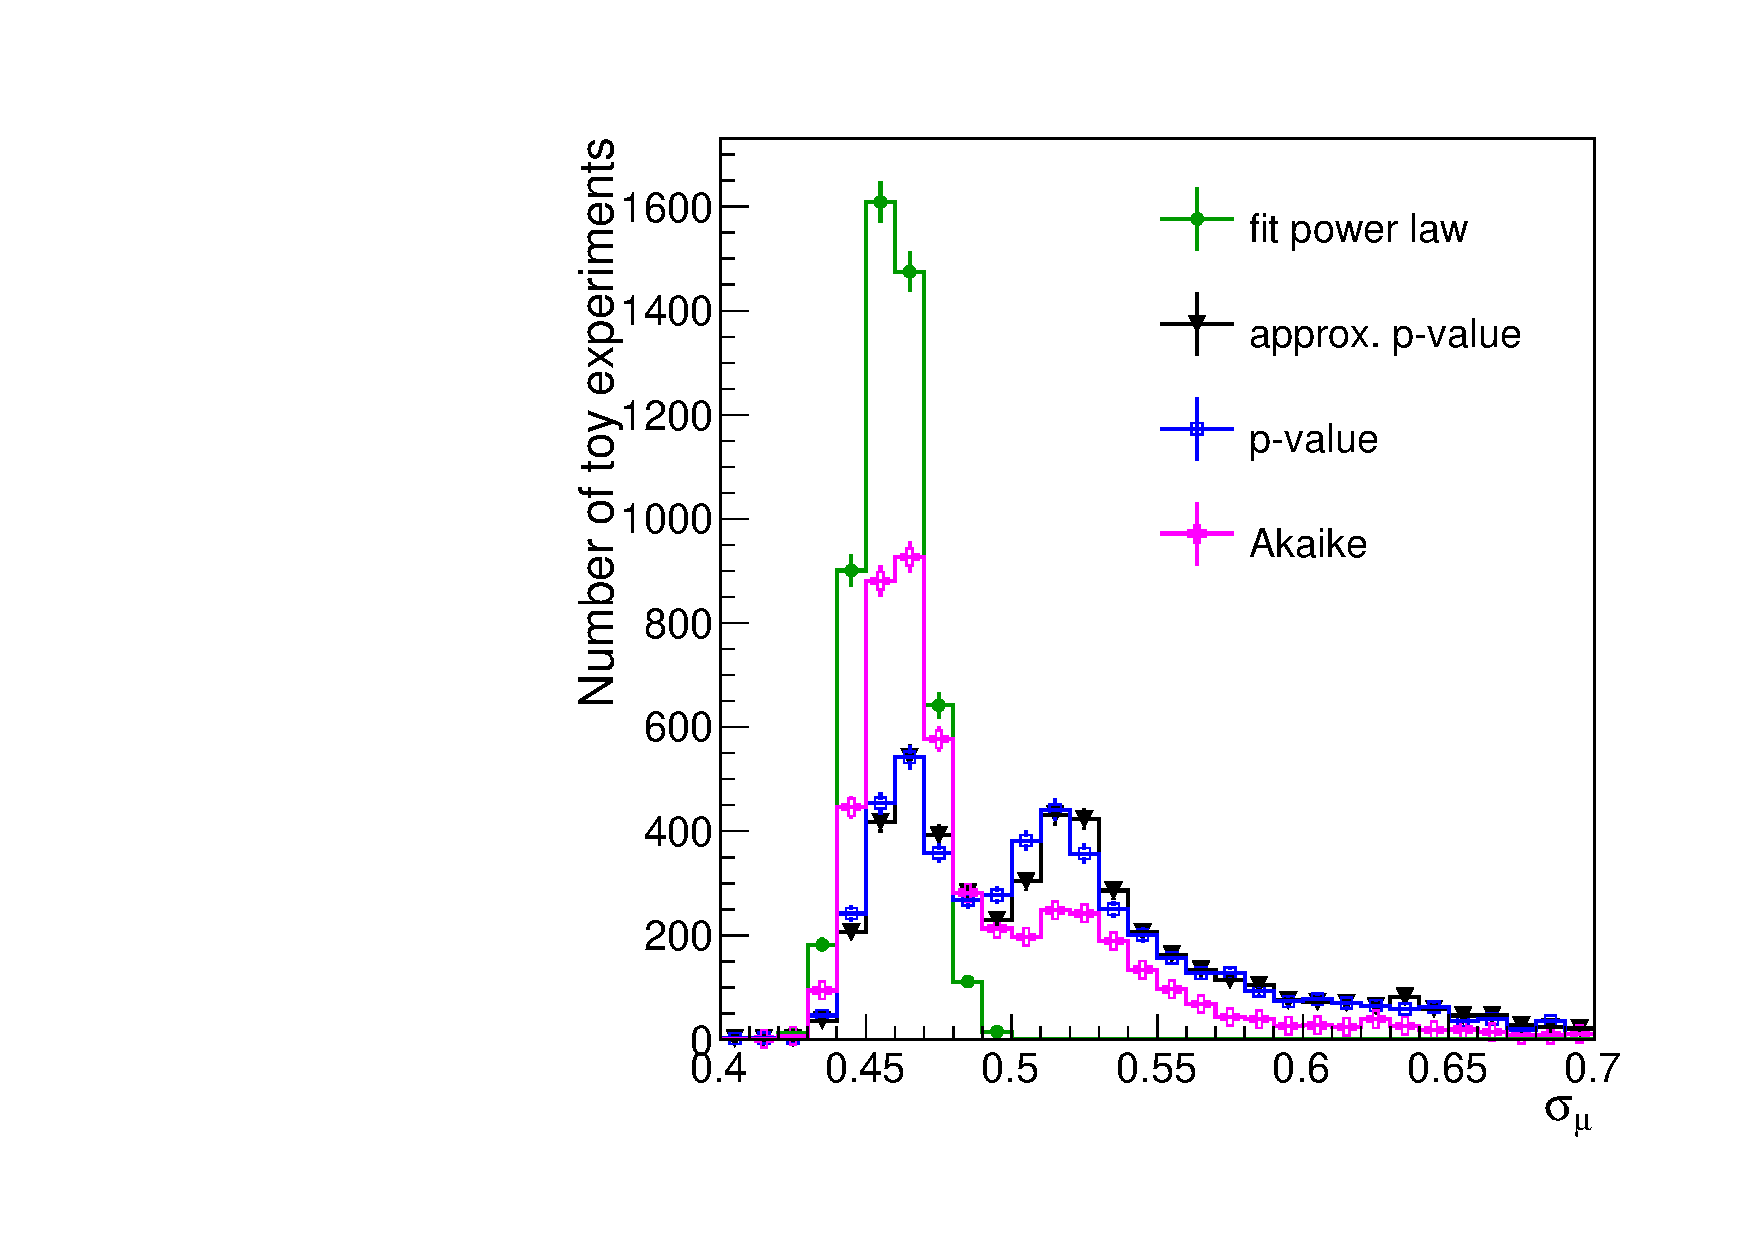
\includegraphics[width=0.45\textwidth]{correction/compare_error_magnitude.pdf}
\caption{Distribution of $\sigma_{\mu}$ in toy datasets
comparing the three correction schemes
when including the full set of functions
to the case when considering only a single power law function
with $N_{\rm par}=2$ for the fit.}
\label{fig:correction:compareerrors}
\end{figure}

%ERROR VS CORRECTION.

%DOES BIAS $\rightarrow 0$ for CORRECTION $\rightarrow 0$?
